%% ======================================== Categorization ===========================

\subsection{Event categorizations}
To improve the sensitivity of search in both VBF and ggF production mode in NWA model, events are classified into the VBF- and ggF- enriched categories.
With the statistic increasing in full run-2 data, a multivariate (MVA) based classifier has been studied for NWA signal, 
while in the meantime the traditional cut-based classifier is also used as a model-independent result for all three (NWA, LWA, graviton) models.

\subsubsection{Cut-based categorization}
There are four categories in total: one VBF-enriched category and three ggF-enriched categories.
The categorization is defined based on kinematic cuts:
\begin{itemize}
	\item VBF-CBA-enriched category: Events have at least two selected jets as defined in section~\ref{sec:hmhzz_objsel}, with the two leading jets being separated by $|\Delta \eta_{jj}| > 3.3$ and invariant mass satisfying $\mjj > 400~\gev$;
	\item ggF-CBA-enriched categories: The remaining events that are not classified into VBF-enriched category. Then events are categorized into three channels based on lepton-flavor, namely ggF\_2$e$2$\mu$, ggF\_4$e$ and ggF\_4$\mu$. 
\end{itemize}
where `CBA' stands for the cut-based categorization.

\subsubsection{MVA-based categorization}
In order to target different production modes, two types of classifiers, one dedicate to VBF production while the other one for ggF, have been trained using deep neural network technique.
Details of two classifiers are described as below:

\textbf{DNN models} 

Figure~\ref{fig:dnn_arch} shows the architecture of VBF (left) and ggF (right) network.
The network structure was chosen based on its AUC~\cite{BRADLEY19971145} value from evaluation samples.
The VBF network includes three parts: two recurrent neural networks (RNNs) and one multilayer perceptron (MLP).
The ggF network consists of one RNN and one MLP.

\begin{figure}[htbp]
        \centering
        \subfloat[]{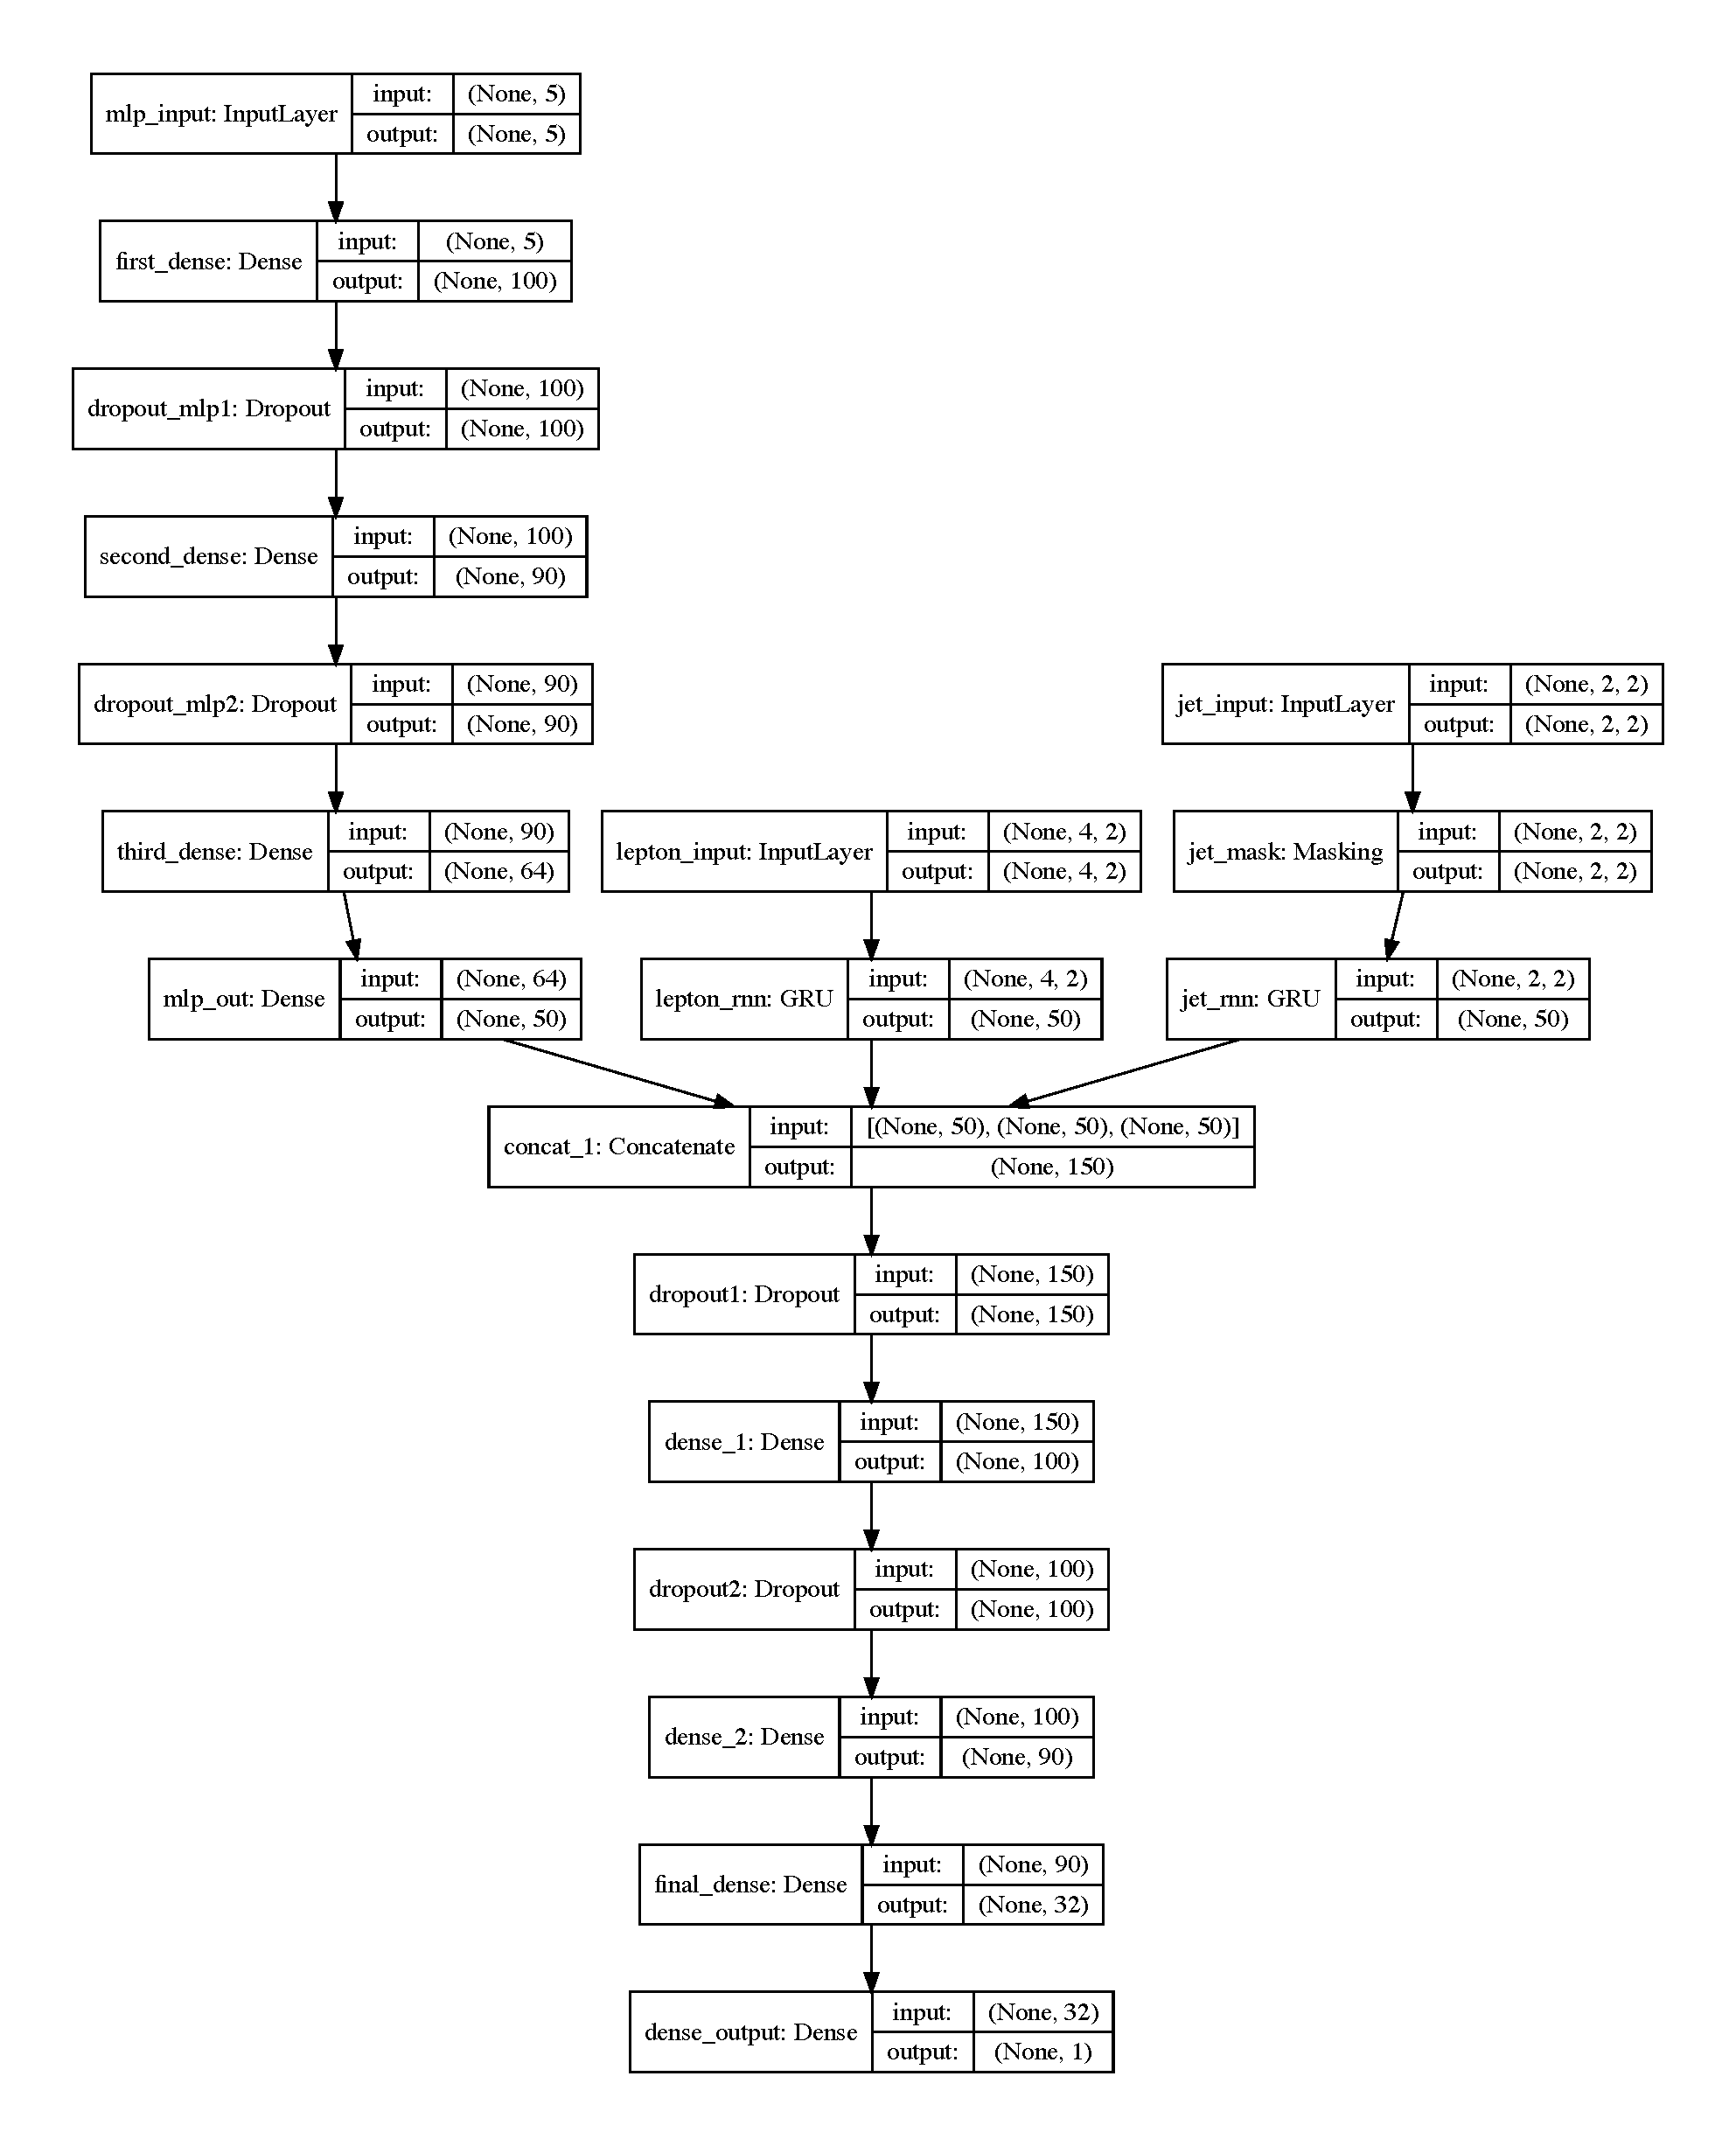
\includegraphics[width=0.49\textwidth]{figures/HMHZZ/selection/model_vbf_architecture.pdf}}
        \subfloat[]{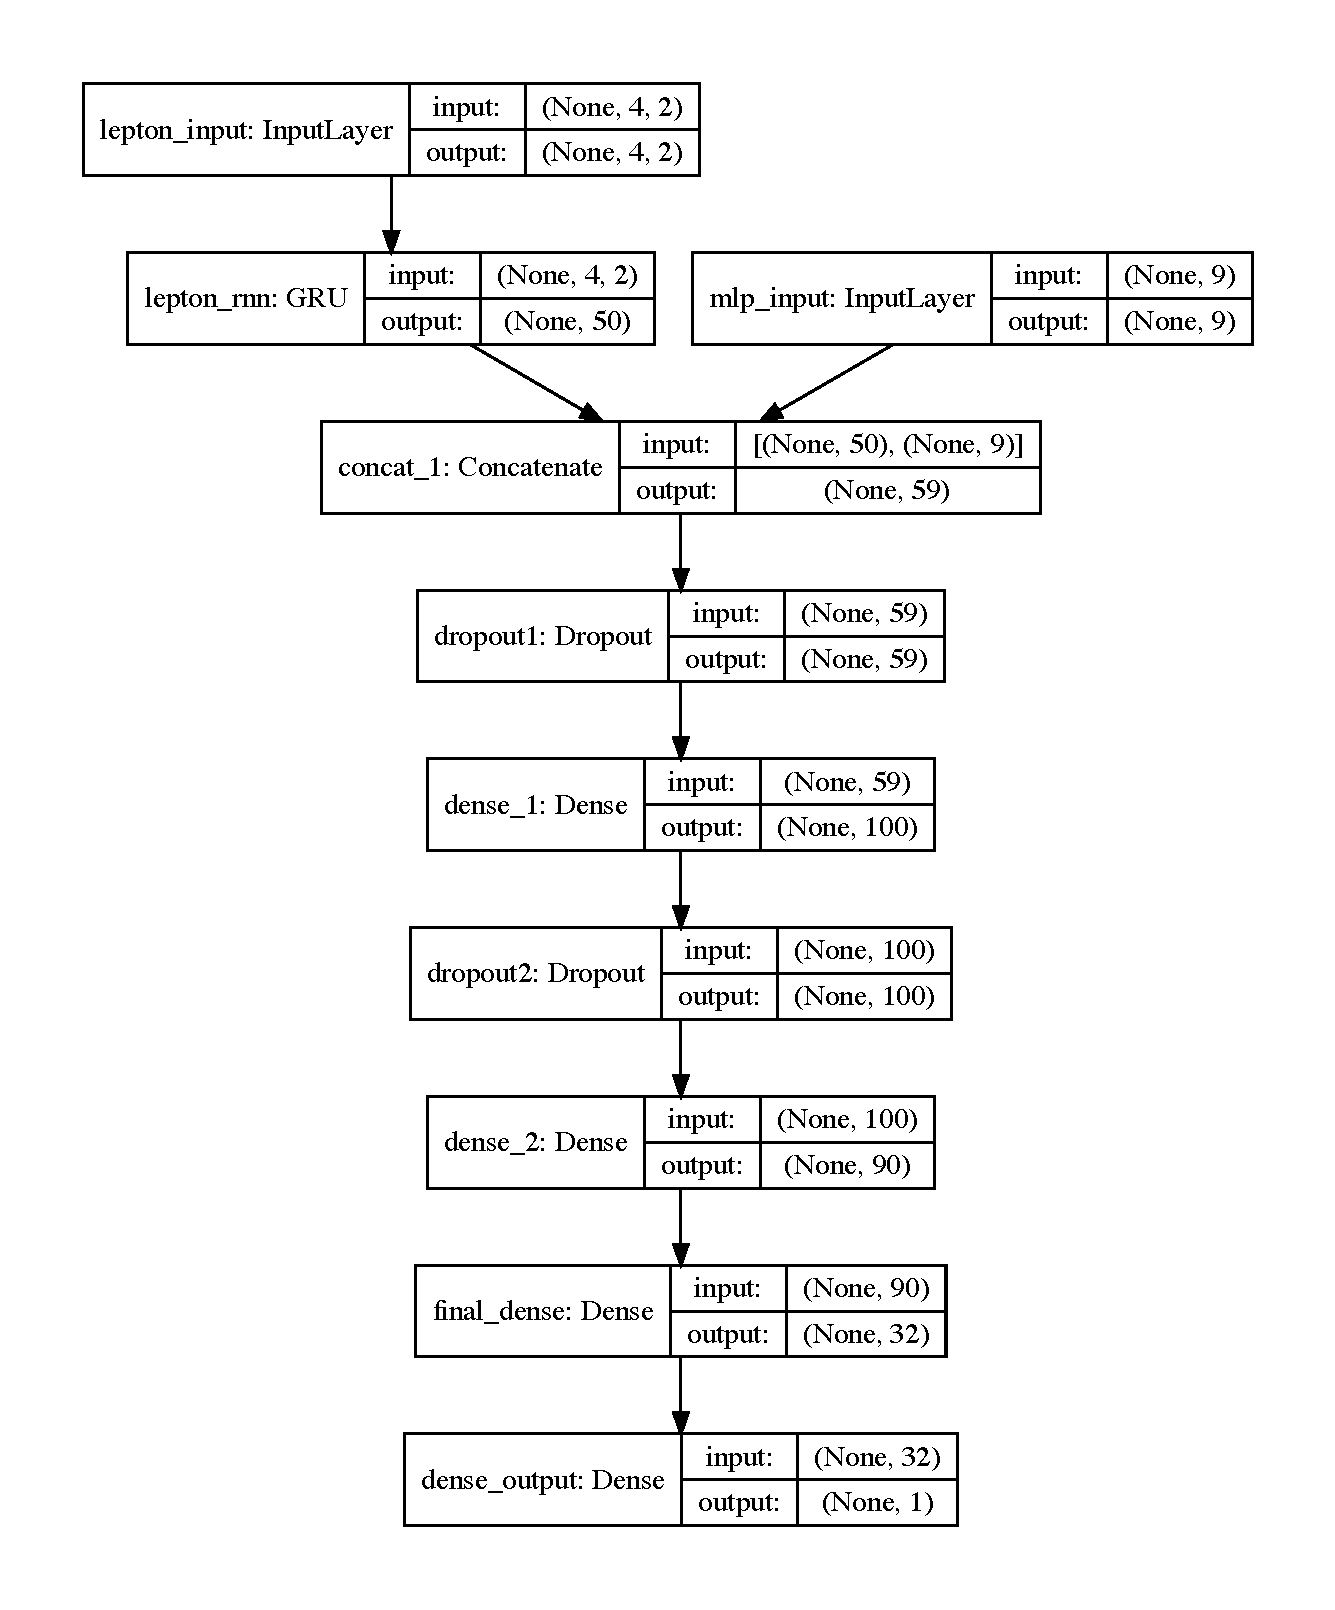
\includegraphics[width=0.49\textwidth]{figures/HMHZZ/selection/model_ggf_architecture.pdf}}
        \caption{(a) VBF DNN architecture diagram. (b) ggF DNN architecture.}
        \label{fig:dnn_arch}
\end{figure}

For training, the VBF and ggF signal samples at the masses of 200, 300, 400, 500, 600, 700, 800, 900, 1000, 1200, 1400~\gev~ are used with positive label.
The VBF (ggF) signals are only used for VBF (ggF) classifier.
The background including simulated samples of QCD and EW \qqZZ processes as well as \ggZZ process summed according to their cross section are assigned with negative labels.
In addition to the selections described in section~\ref{sec:hmhzz_eventsel}, the events used for VBF network are required to have $N_\mathrm{jets} \geq 2$, while $N_\mathrm{jets} < 2$ is required for events in ggF network,
so the training events for two network are independent.

In order to assign equivalent importance to signals with different mass assumptions, during the training, signal events are reweighted to follow the \mfl distribution from background (idea from Ref.~\cite{Baldi:2016fzo} with a modified reweighting procedure), 
as shown in figure~\ref{fig:dnn_rwt_vbf} (figure~\ref{fig:dnn_rwt_ggf}) before and after reweighting for VBF (ggF) samples.

\begin{figure}[htbp]
        \centering
        \subfloat[]{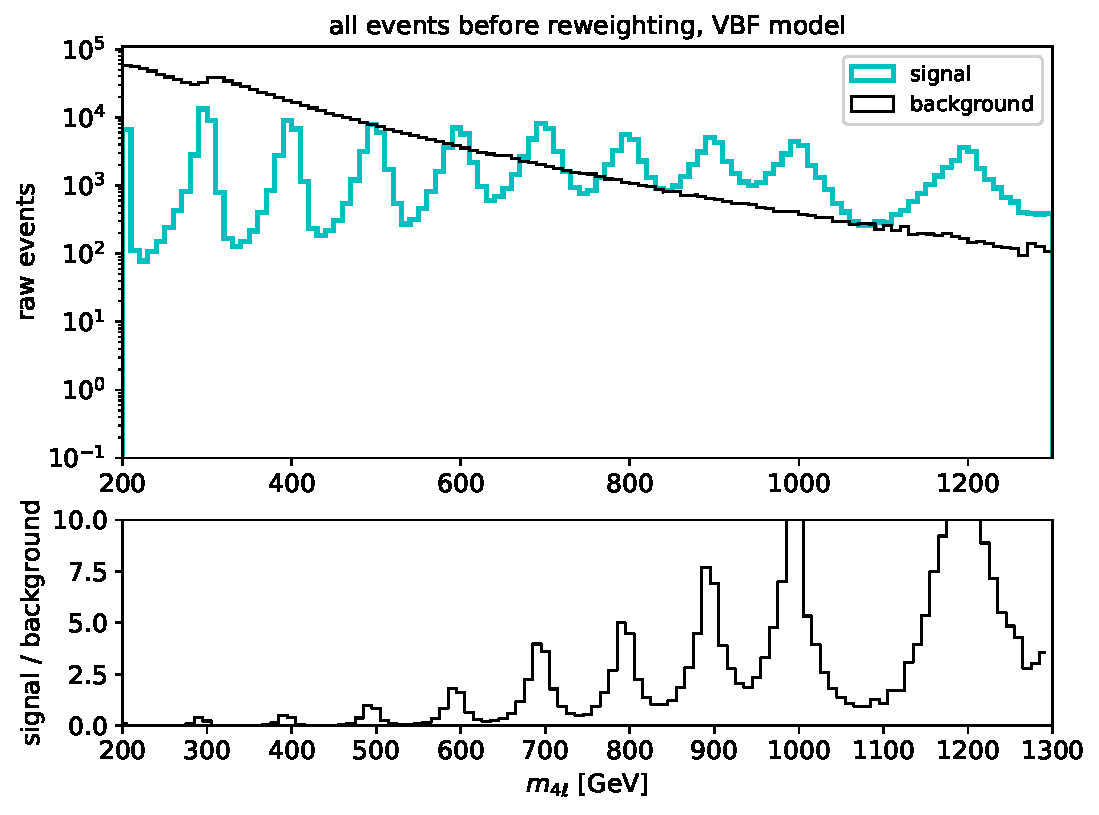
\includegraphics[width=0.48\textwidth]{{figures/HMHZZ/selection/vbf_input/m4l_before_reweighting.pdf}}}
        \subfloat[]{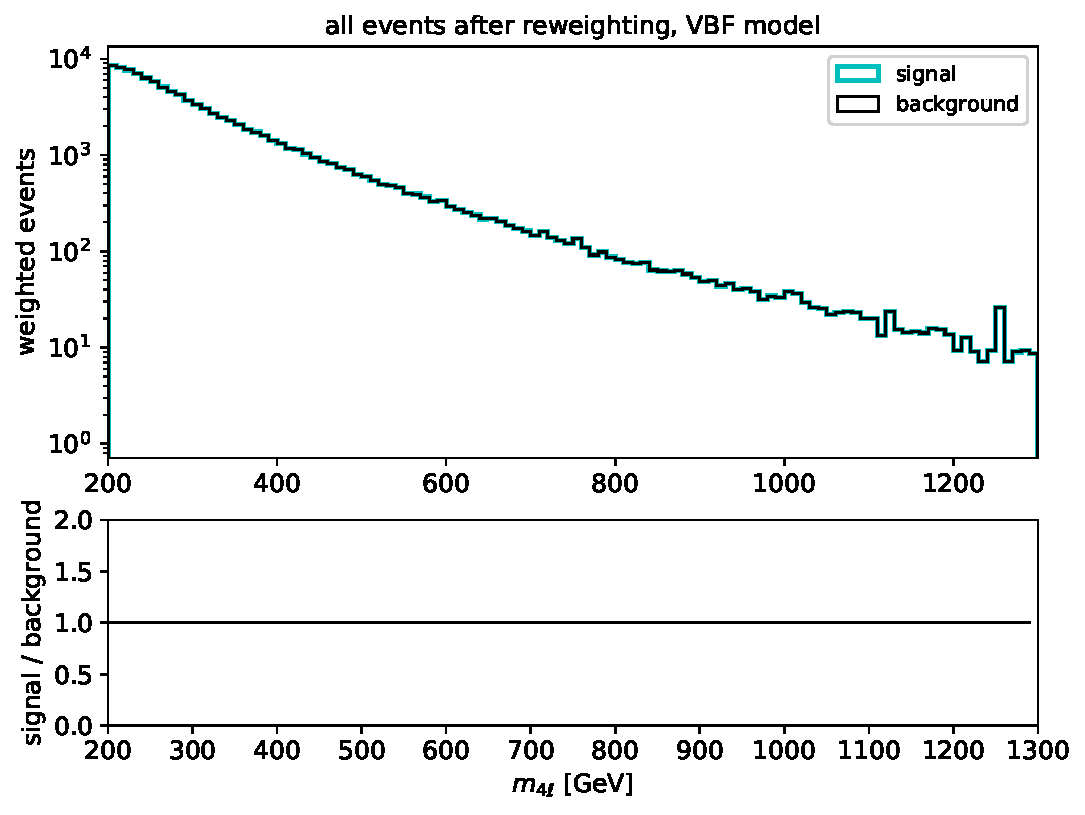
\includegraphics[width=0.48\textwidth]{{figures/HMHZZ/selection/vbf_input/m4l_after_reweighting.pdf}}}
        \caption{(a) \mfl distribution of raw (unweighted) training events for VBF signal (blue) and background (black); (b) \mfl distribution of weighted VBF signal (blue) and background (black) used at training time.}
        \label{fig:dnn_rwt_vbf}
\end{figure}

\begin{figure}[htbp]
        \centering
        \subfloat[]{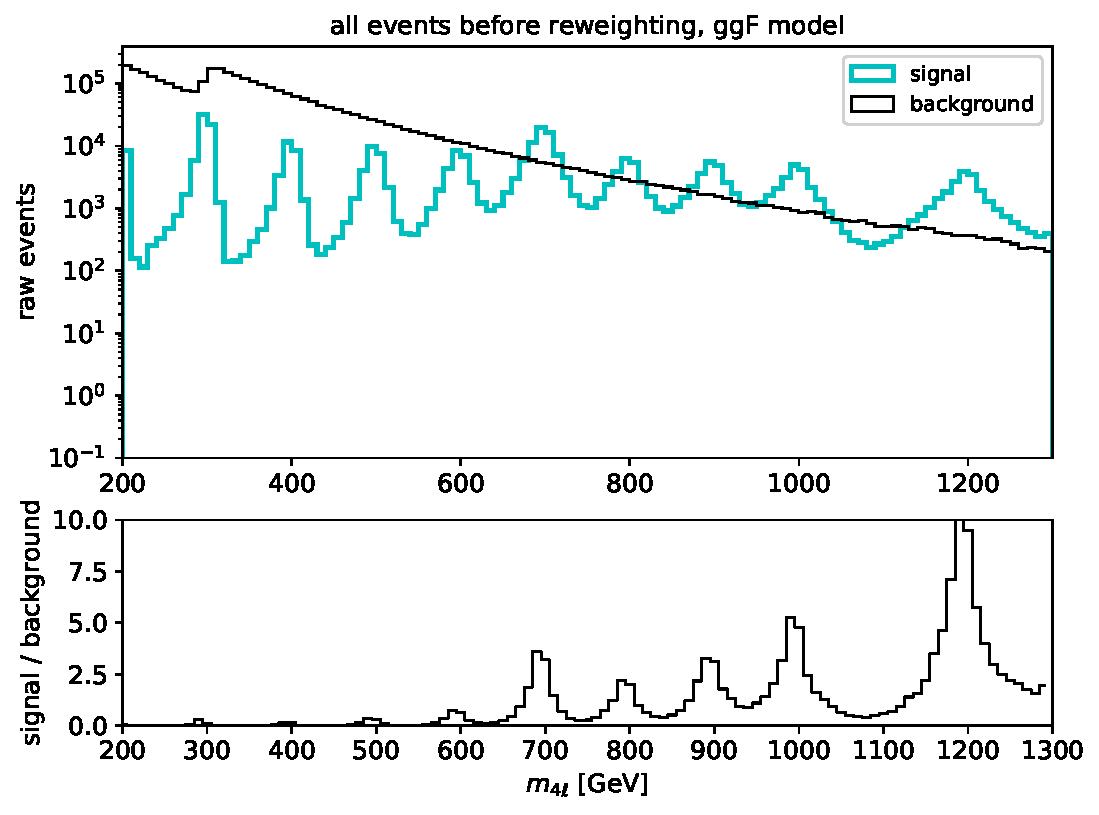
\includegraphics[width=0.48\textwidth]{{figures/HMHZZ/selection/ggf_input/m4l_all_before_reweighting.pdf}}}
        \subfloat[]{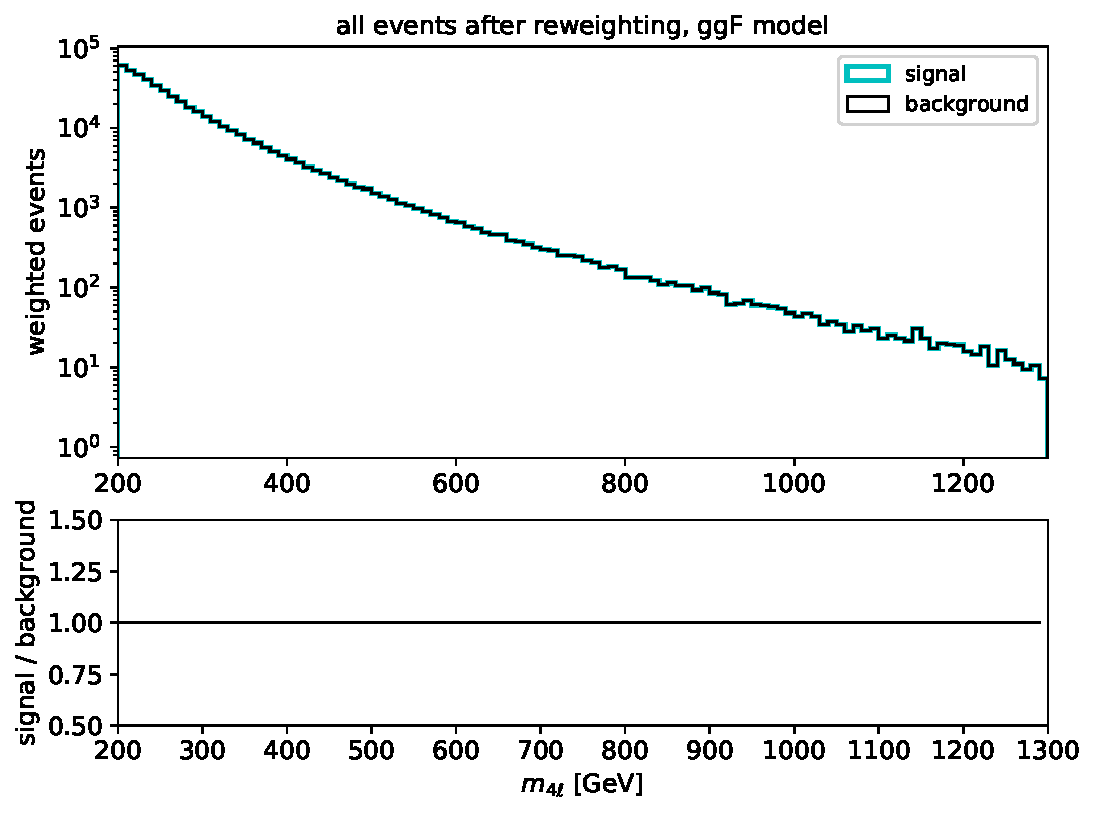
\includegraphics[width=0.48\textwidth]{{figures/HMHZZ/selection/ggf_input/m4l_all_after_reweighting.pdf}}}
        \caption{(a) \mfl distribution of raw (unweighted) training events for ggF signal (blue) and background (black); (b) \mfl distribution of weighted ggF signal (blue) and background (black) used at training time.}
        \label{fig:dnn_rwt_ggf}
\end{figure}

%After all these preparation, then the training is performed over 20 epochs with batch size of 512 (256) for VBF (ggF) network.


\textbf{Input features}

Table~\ref{tab:dnn_features_VBF} (table~\ref{tab:dnn_features_ggF}) lists the input features used for VBF (ggF) network during the training.
For VBF network, one RNN (the other one) takes the \pt and $\eta$ of \pt-ordered four leptons (two leading jets) as input features, which intends to study the time relationship from particle decay between leptons (jets).
For ggF network, the only one RNN model takes the \pt and $\eta$ of \pt-ordered four leptons as inputs.

\begin{table}
\caption{
Input features used in the ``VBF-classifier'' for the \llll analysis.
The RNN stands for the recurrent neural network and MLP for the multilayer perceptron.
\label{tab:dnn_features_VBF}}
\centering
\begingroup
\setlength{\tabcolsep}{10pt}
\renewcommand{\arraystretch}{1.0}
\begin{tabularx}{\textwidth}{ccX}
\toprule
Model &    Inputs                                & Description \\ \hline
\multirow{4}{*}{RNN}    & $\pt^{\text{j0}, \text{j1}}$            & transverse momenta of the two leading jets \\
                        & $\eta^{\text{j0}, \text{j1}}$           & pseudorapidity of the two leading jets \\
                        & $\pt^{\ell0, \ell1, \ell2, \ell3}$      & transverse momenta of the four leptons \\
                        & $\eta^{\ell0, \ell1, \ell2, \ell3}$     & pseudorapidity of the four leptons \\
                        \midrule
\multirow{5}{*}{MLP}    & \mfl                          & invariant mass of the four lepton system \\
                        & \mjj                          & invariant mass of the two leading jet system \\
                        & $\pt^{\text{jj}}$             & transverse momentum of the two leading jet system \\
                        & $\Delta\eta_{\text{H,j}}$     & difference in pseudorapidity between the four lepton system and the leading jet \\
                        & min$\Delta R_{\text{jZ}}$     & minimum distance between one of the two lepton pairs and a jet \\

\bottomrule
\end{tabularx}
\endgroup
\end{table}

\begin{table}
    \caption{
    Input features used in the ``ggF-classifier'' for the \llll analysis.
    The RNN stands for the recurrent neural network and MLP for the multilayer perceptron.
    \label{tab:dnn_features_ggF}}
    \centering
\begingroup
\setlength{\tabcolsep}{10pt}
\renewcommand{\arraystretch}{1.0}
\begin{tabularx}{\textwidth}{ccX}
\toprule
Model & Inputs                                & Description \\ \hline
\multirow{2}{*}{RNN}    & $\pt^{\ell0, \ell1, \ell2, \ell3}$      & transverse momenta of the four leptons \\
                        & $\eta^{\ell0, \ell1, \ell2, \ell3}$     & pseudorapidity of the four leptons \\
\midrule
\multirow{9}{*}{MLP}    & \mfl                & invariant mass of the four lepton system \\
                        & $\pt^{4\ell}$       & transverse momentum of the four lepton system \\
                        & $\eta^{4\ell}$      & pseudorapidity of the four lepton system \\
                        & $\cos\theta^*$      & production angle of the leading $Z$ defined in the four lepton rest frame \\
                        & $\cos\theta_{1}$    & angle between the negative final state lepton and the direction of flight of leading $Z$ in the $Z$ rest frame \\
                        & $\cos\theta_{2}$    & angle between the negative final state lepton and the direction of flight of sub-leading $Z$ in the $Z$ rest frame \\
                        & $\Phi$              & angle between the decay planes of the four final state leptons expressed in the four lepton rest frame \\
                        & $\pt^{\text{j0}}$   & transverse momentum of the leading jet \\
                        & $\eta^{\text{j0}}$  & pseudorapidity of the leading jet \\

\bottomrule
    \end{tabularx}
    \endgroup
    \end{table}


%Figure~\ref{fig:dnn_vbf_distribution} (figure~\ref{fig:dnn_ggf_distribution}) shows the distributions of input features with events before training reweighting for VBF (ggF) network of background and 4 signal samples at mass points of 300, 700, 1400 and 2000~\gev.
%
%\begin{figure}[htbp]
%        \captionsetup[subfigure]{labelformat=empty}
%        \centering
%        \subfloat[]{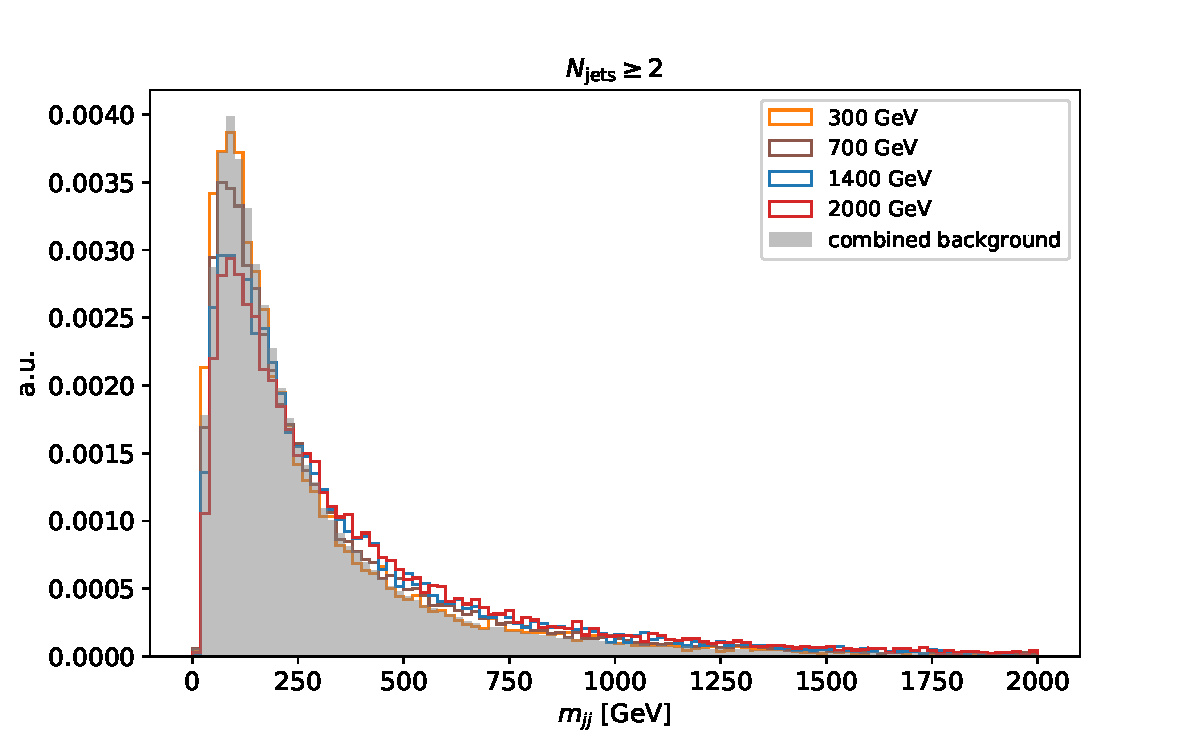
\includegraphics[width=0.19\textwidth]{figures/HMHZZ/selection/vbf_input/input_comparison_300_to_2000_0_score_dijet_invmass}}
%        \subfloat[]{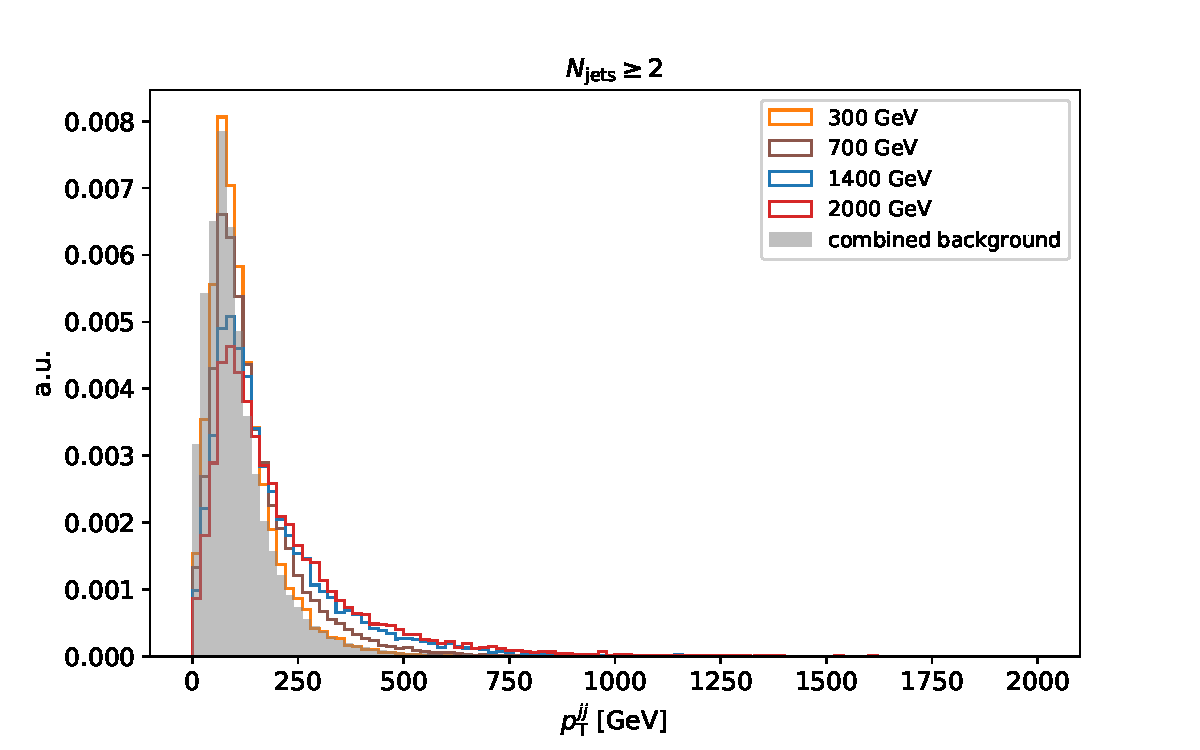
\includegraphics[width=0.19\textwidth]{figures/HMHZZ/selection/vbf_input/input_comparison_300_to_2000_2_score_dijet_pt}}
%        \subfloat[]{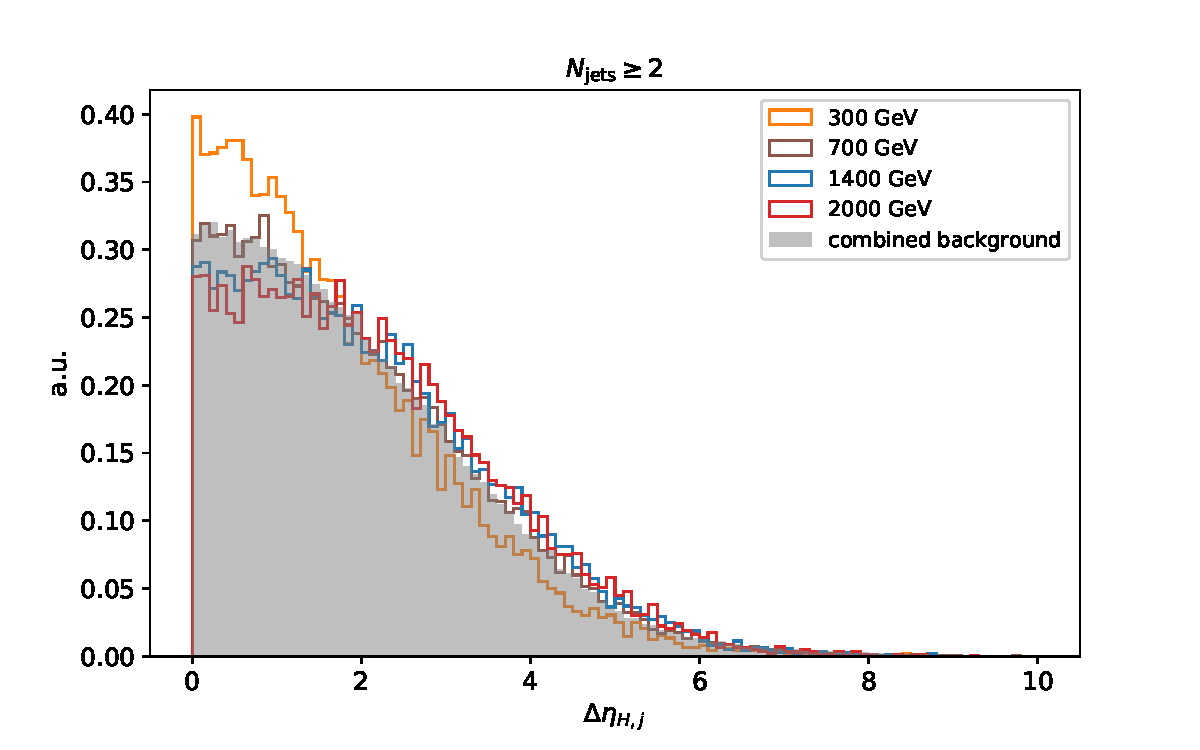
\includegraphics[width=0.19\textwidth]{figures/HMHZZ/selection/vbf_input/input_comparison_300_to_2000_3_score_eta_zepp_ZZ}}
%        \subfloat[]{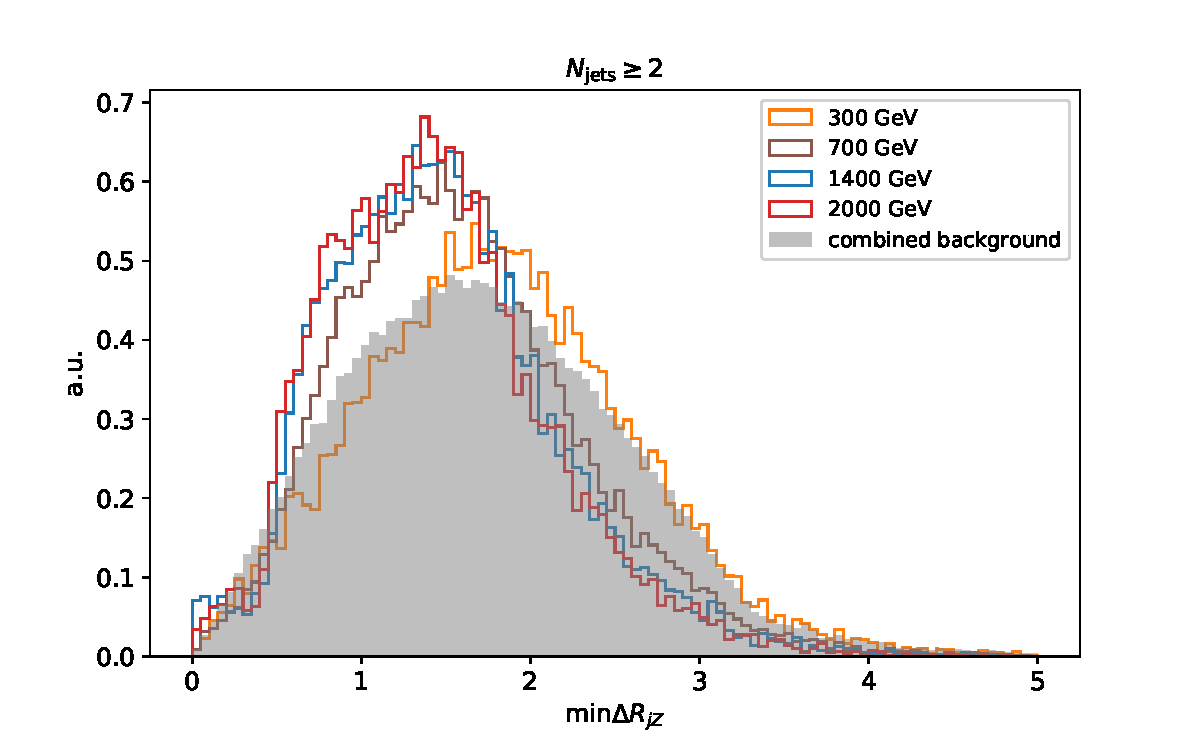
\includegraphics[width=0.19\textwidth]{figures/HMHZZ/selection/vbf_input/input_comparison_300_to_2000_4_score_min_dR_jZ}}
%        \subfloat[]{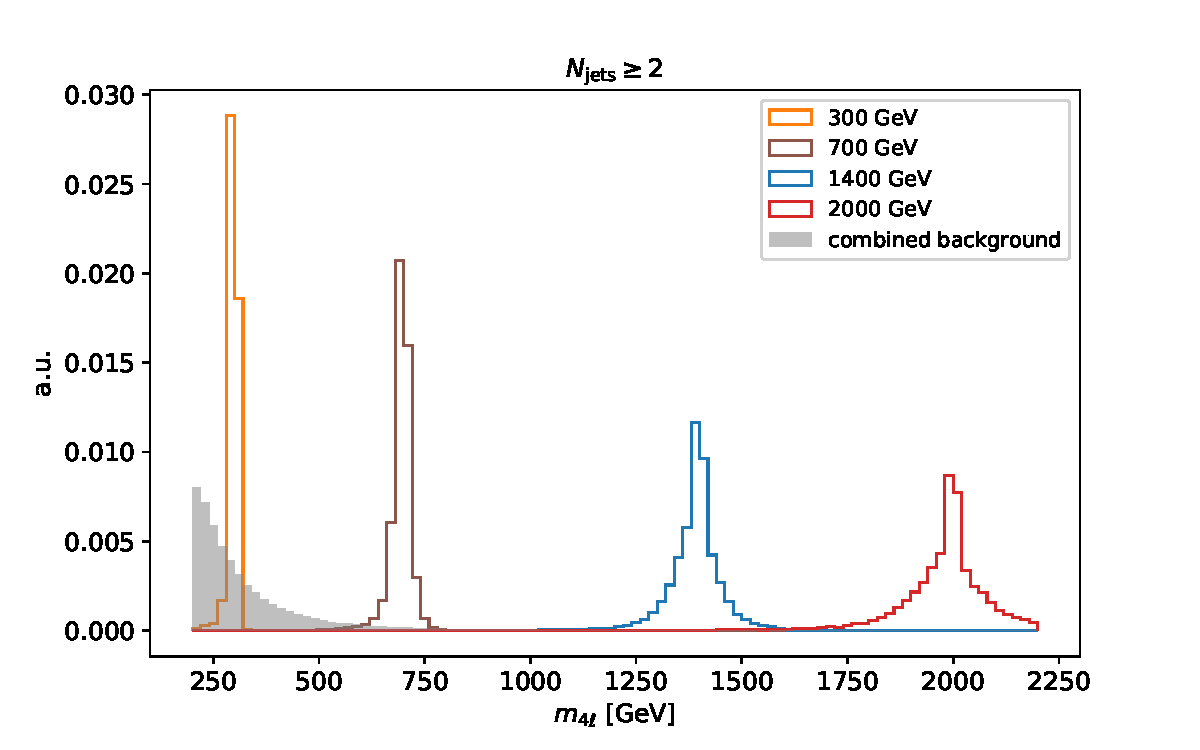
\includegraphics[width=0.19\textwidth]{figures/HMHZZ/selection/vbf_input/input_comparison_300_to_2000_5_score_m4l_unconstrained}}\\
%
%        \subfloat[]{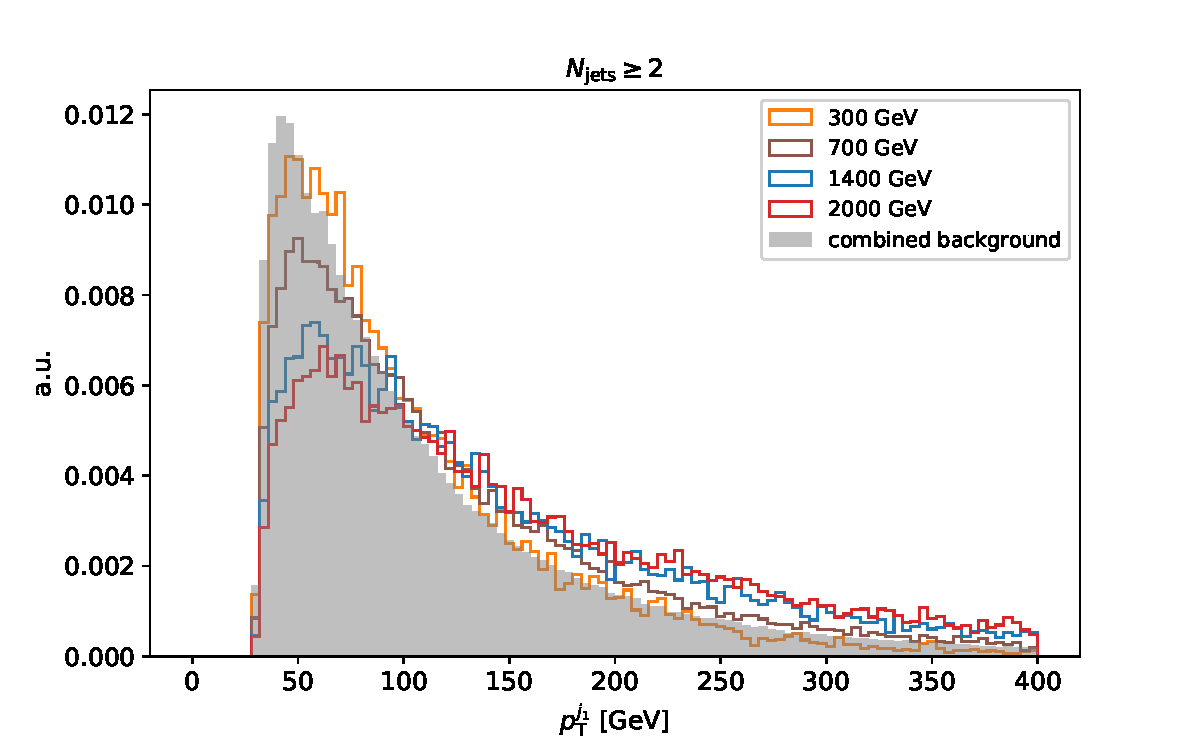
\includegraphics[width=0.24\textwidth]{figures/HMHZZ/selection/vbf_input/input_comparison_300_to_2000_23_score_j_1_pt}}
%        \subfloat[]{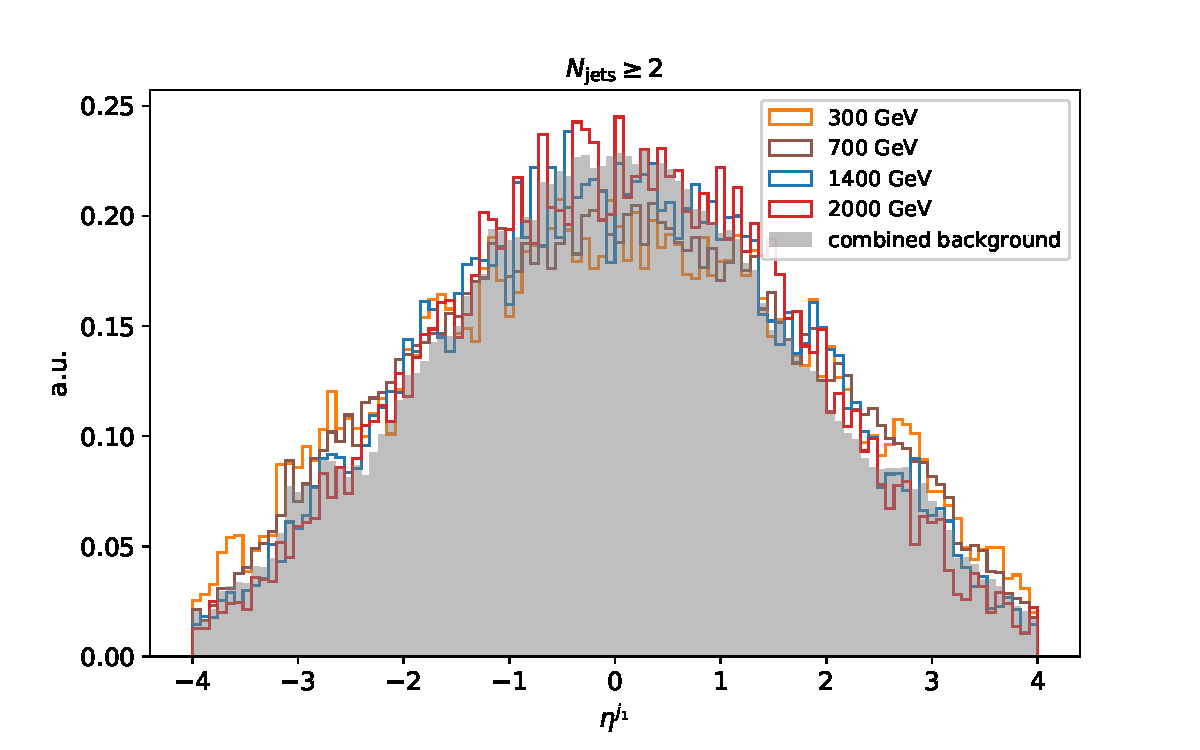
\includegraphics[width=0.24\textwidth]{figures/HMHZZ/selection/vbf_input/input_comparison_300_to_2000_24_score_j_1_eta}}
%        \subfloat[]{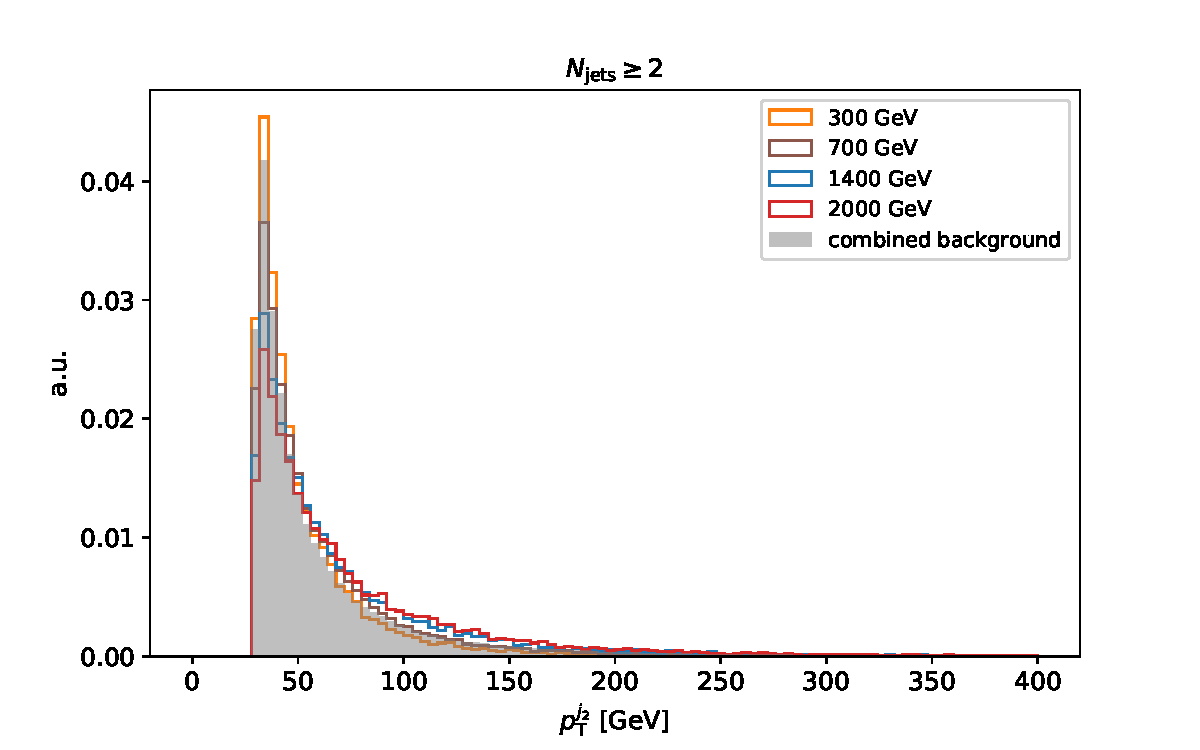
\includegraphics[width=0.24\textwidth]{figures/HMHZZ/selection/vbf_input/input_comparison_300_to_2000_25_score_j_2_pt}}
%        \subfloat[]{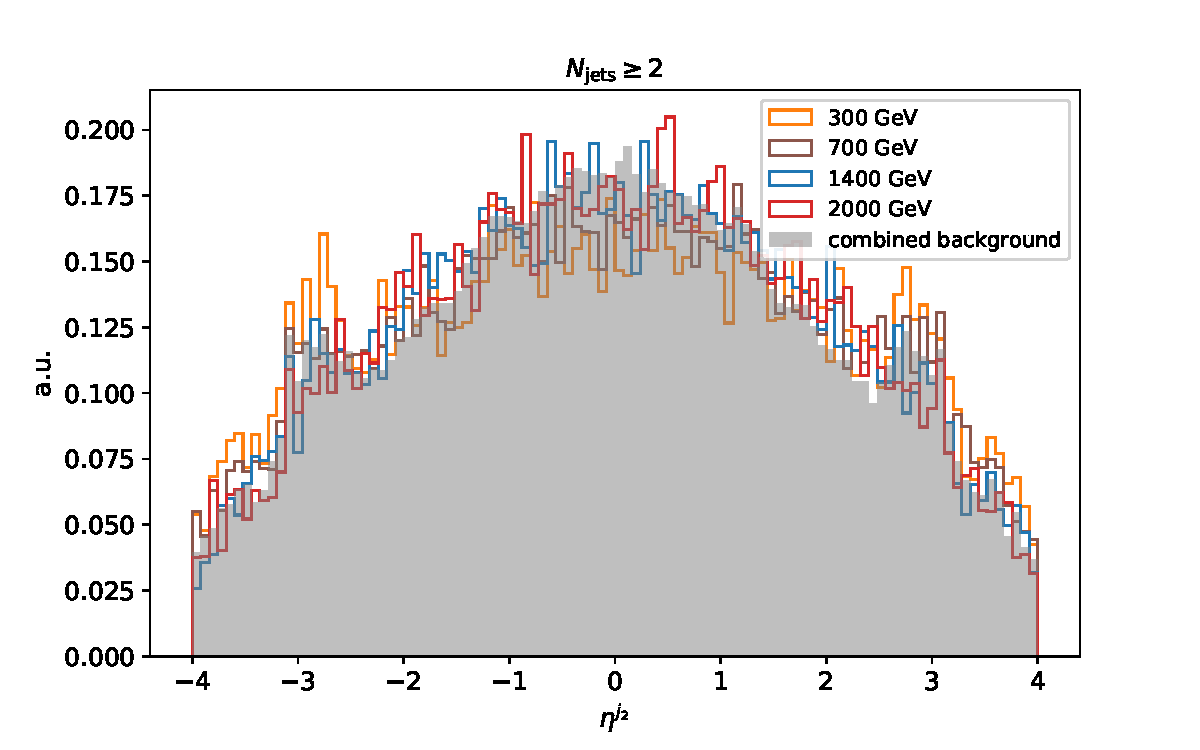
\includegraphics[width=0.24\textwidth]{figures/HMHZZ/selection/vbf_input/input_comparison_300_to_2000_26_score_j_2_eta}}\\
%
%        \subfloat[]{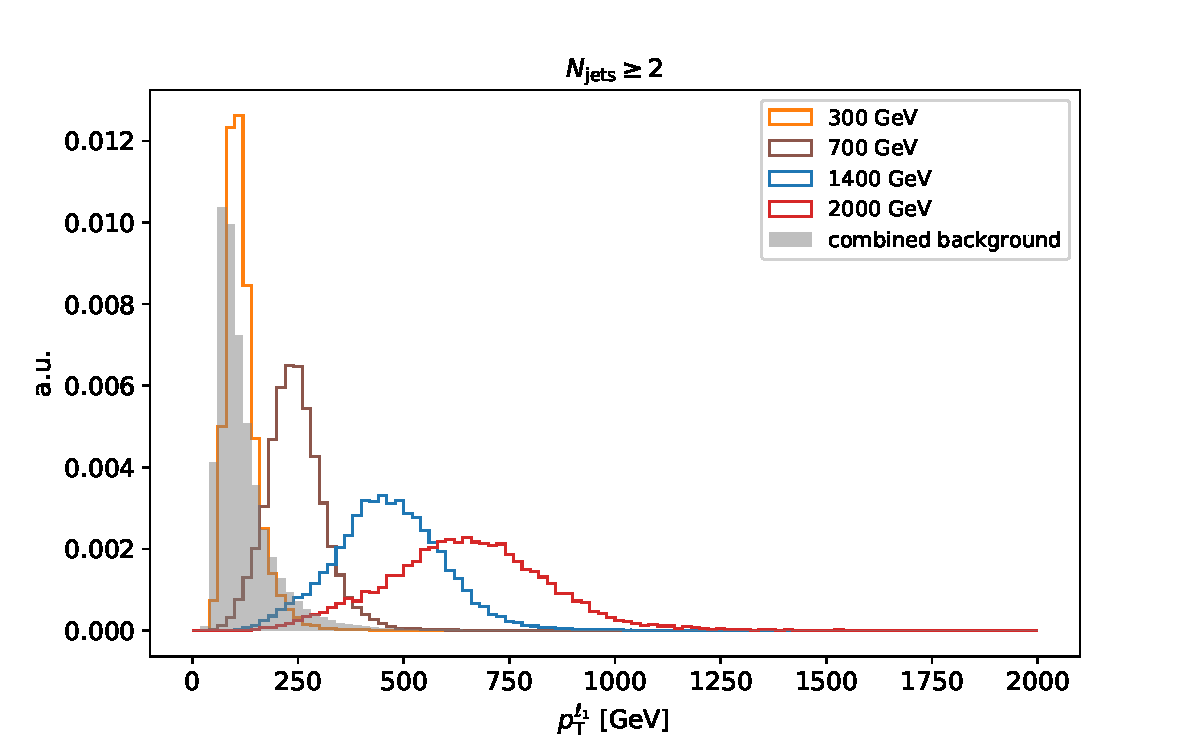
\includegraphics[width=0.24\textwidth]{figures/HMHZZ/selection/vbf_input/input_comparison_300_to_2000_15_score_lep_1_pt}}
%        \subfloat[]{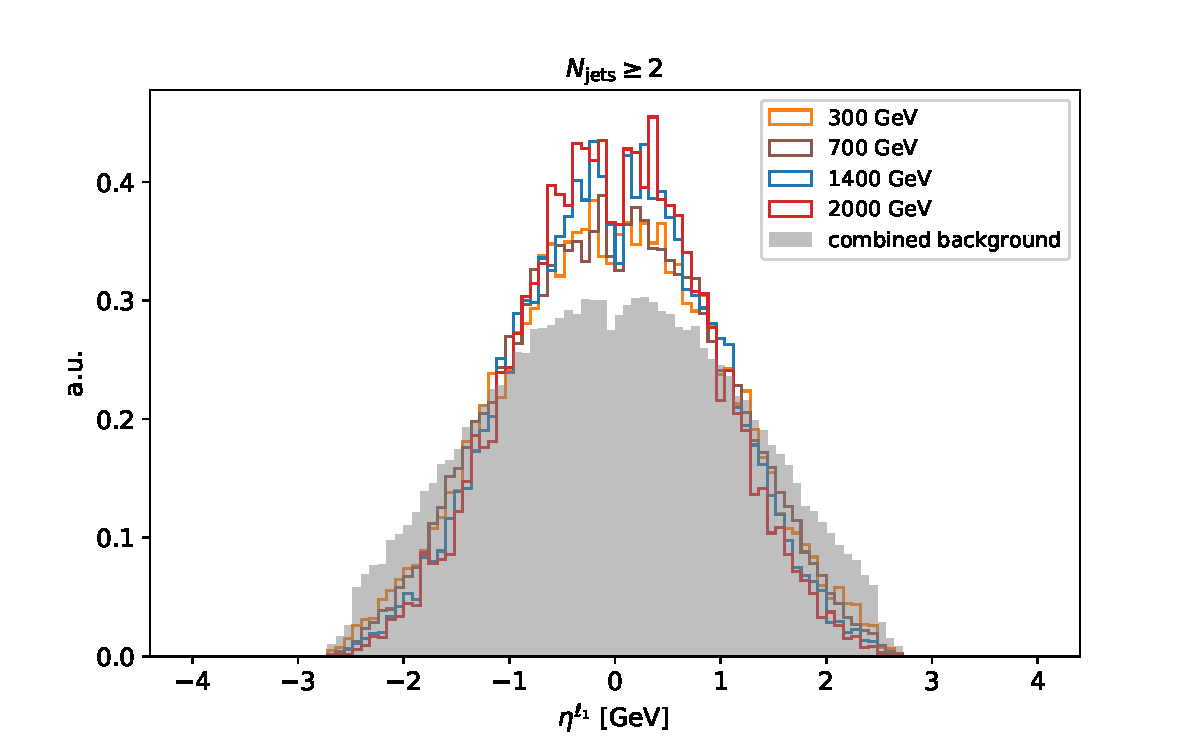
\includegraphics[width=0.24\textwidth]{figures/HMHZZ/selection/vbf_input/input_comparison_300_to_2000_16_score_lep_1_eta}}
%        \subfloat[]{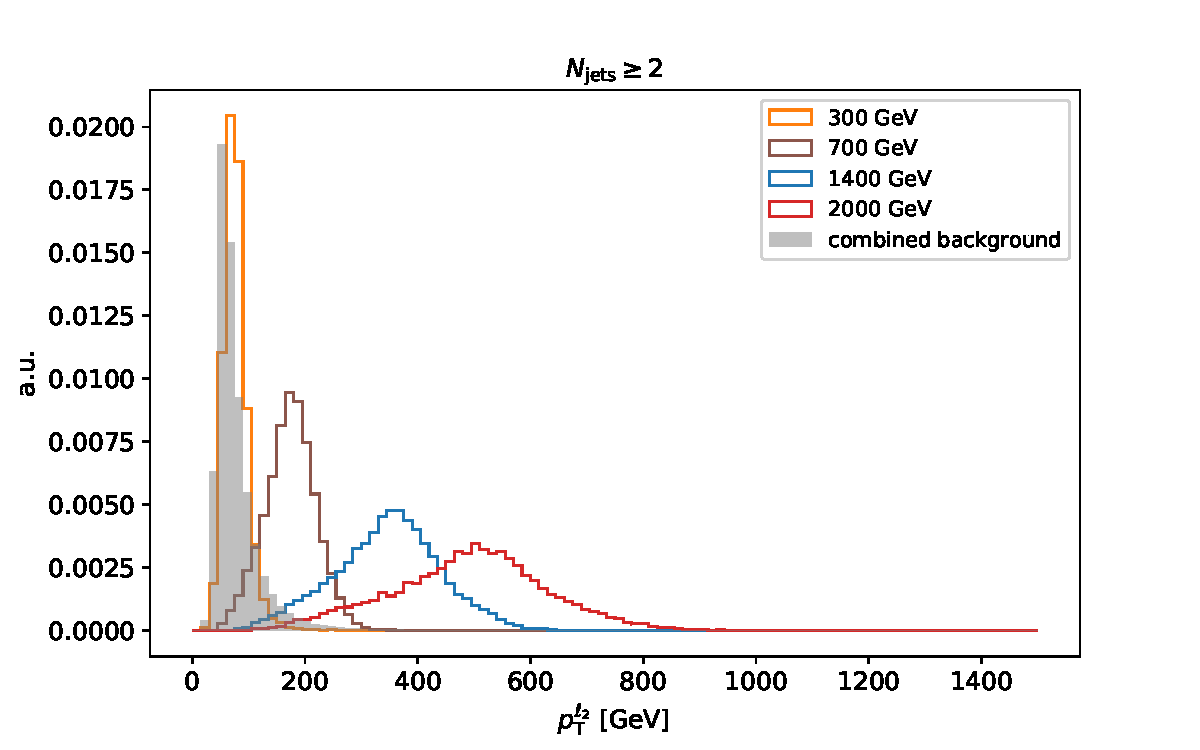
\includegraphics[width=0.24\textwidth]{figures/HMHZZ/selection/vbf_input/input_comparison_300_to_2000_17_score_lep_2_pt}}
%        \subfloat[]{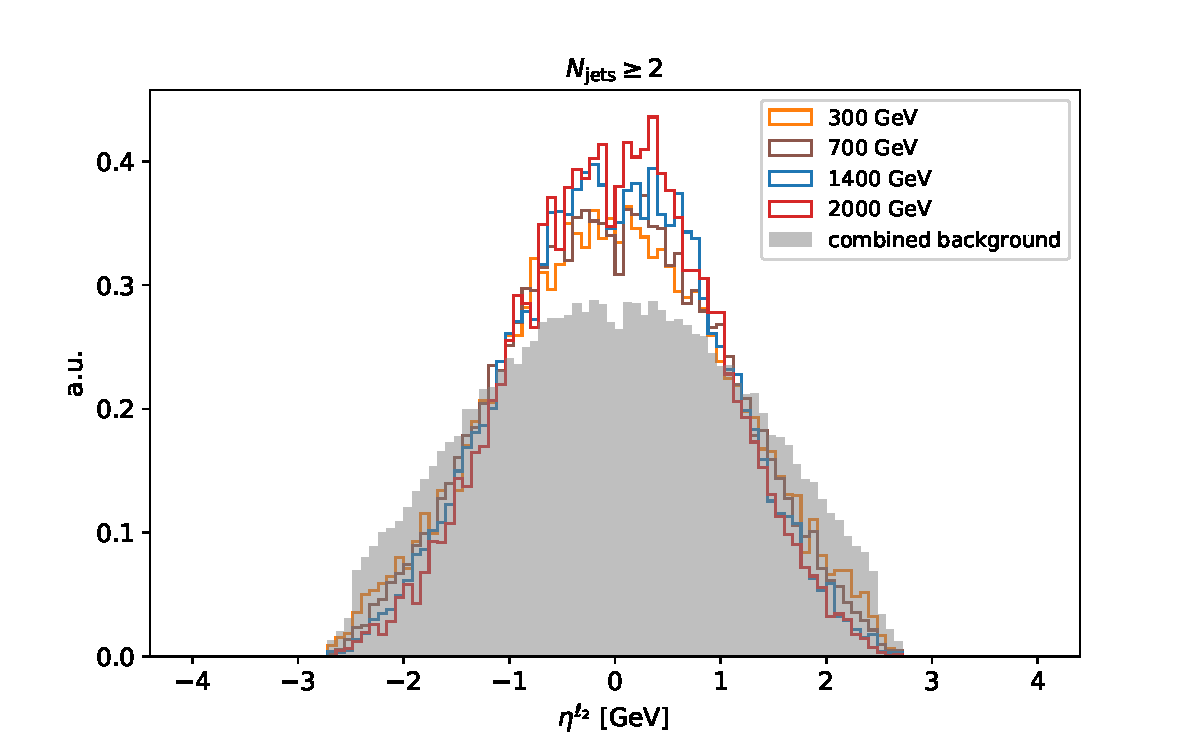
\includegraphics[width=0.24\textwidth]{figures/HMHZZ/selection/vbf_input/input_comparison_300_to_2000_18_score_lep_2_eta}}\\
%
%        \subfloat[]{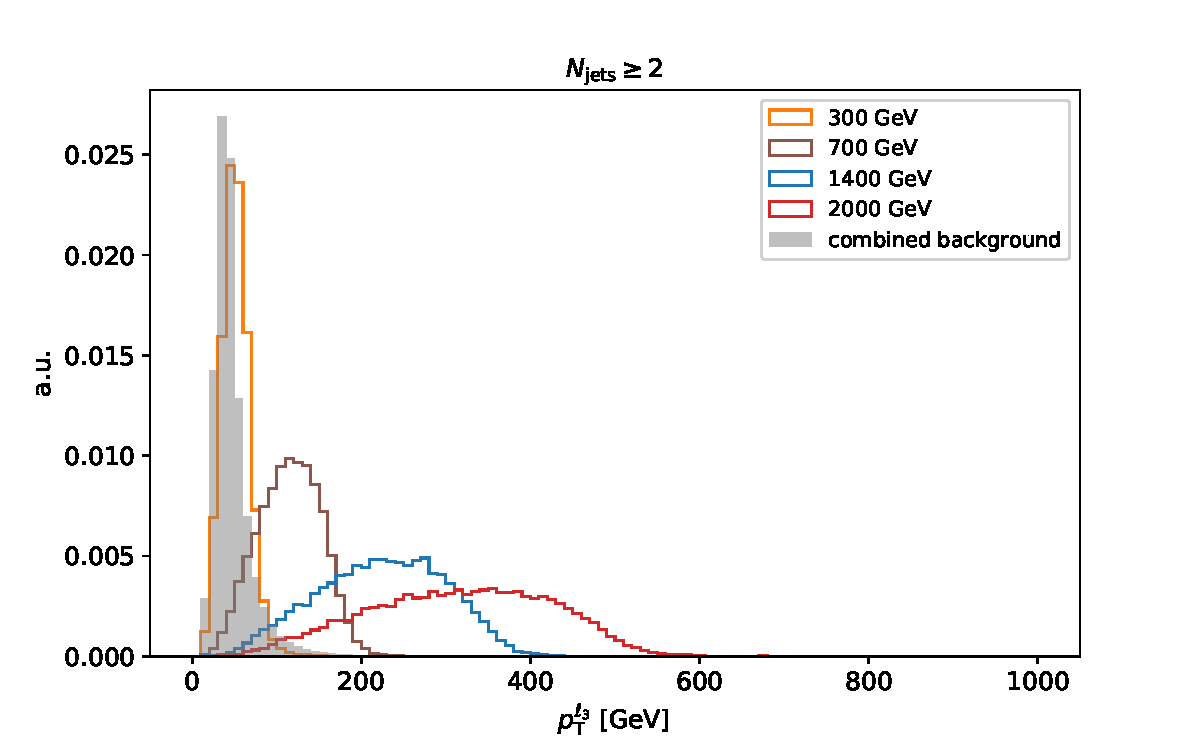
\includegraphics[width=0.24\textwidth]{figures/HMHZZ/selection/vbf_input/input_comparison_300_to_2000_19_score_lep_3_pt}}
%        \subfloat[]{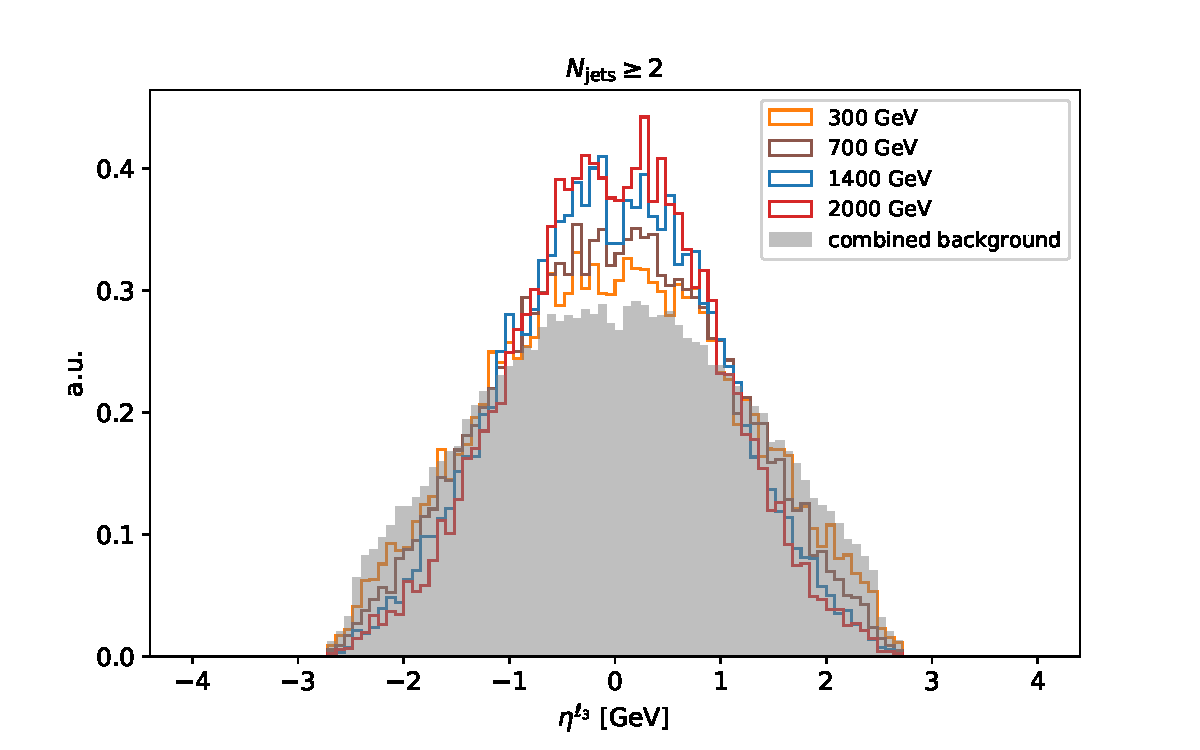
\includegraphics[width=0.24\textwidth]{figures/HMHZZ/selection/vbf_input/input_comparison_300_to_2000_20_score_lep_3_eta}}
%        \subfloat[]{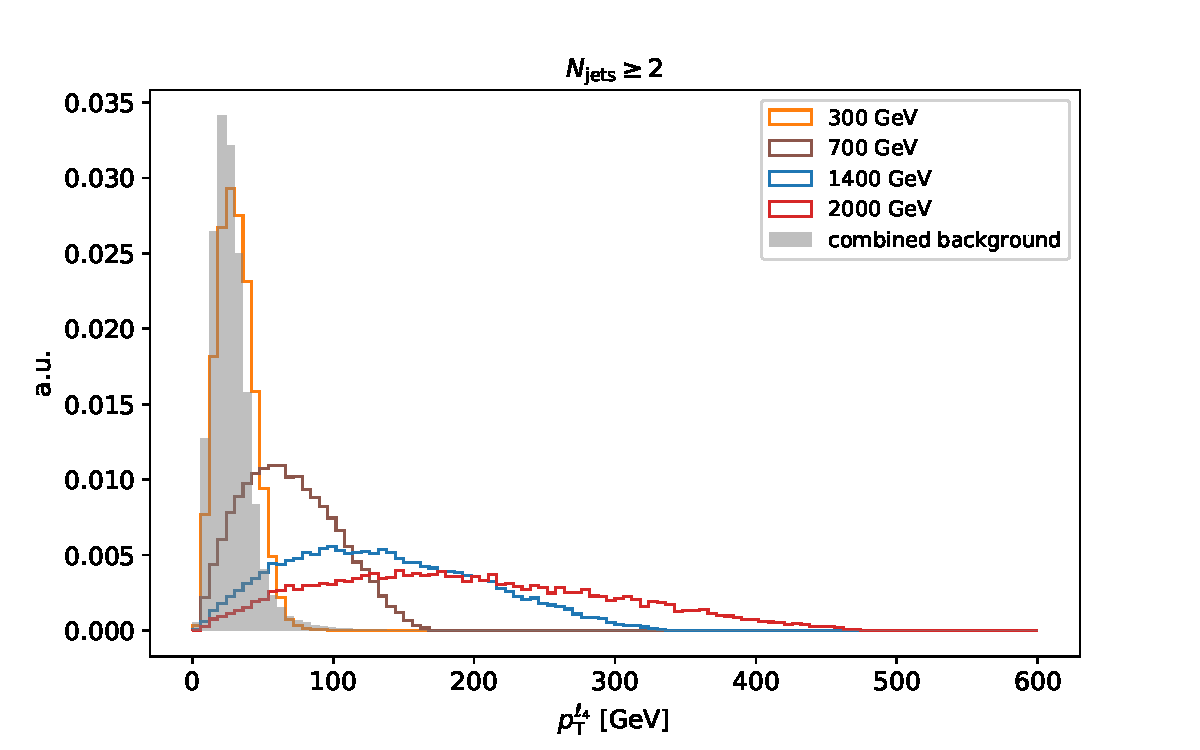
\includegraphics[width=0.24\textwidth]{figures/HMHZZ/selection/vbf_input/input_comparison_300_to_2000_21_score_lep_4_pt}}
%        \subfloat[]{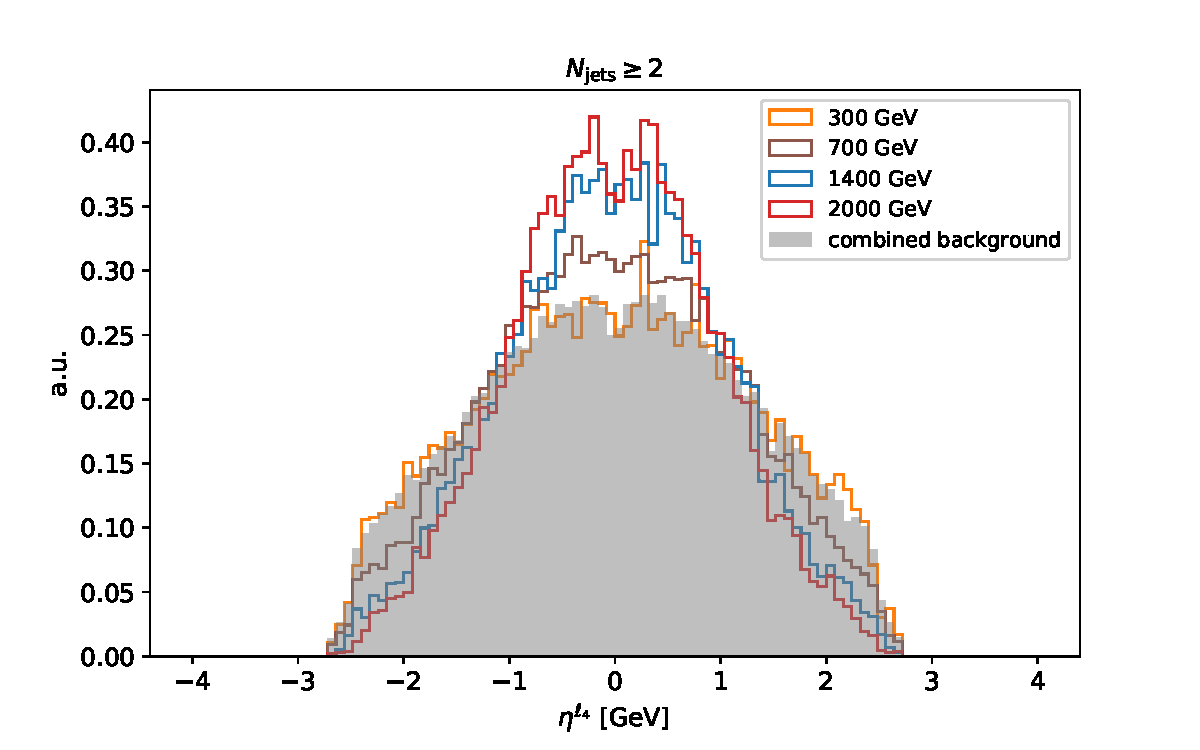
\includegraphics[width=0.24\textwidth]{figures/HMHZZ/selection/vbf_input/input_comparison_300_to_2000_22_score_lep_4_eta}}\\
%        \caption{Distributions of input features as listed in table~\ref{tab:dnn_features_vbf} for the VBF network of signals at mass points of 300, 700, 1400, 2000~\gev (coloured) and the background (grey). Only events satisfying the training selection of $N_\mathrm{jets}\geq2$ are shown.}
%        \label{fig:dnn_vbf_distribution}
%\end{figure}

%\begin{figure}[htbp]
%        \centering
%        \captionsetup[subfigure]{labelformat=empty}
%        \subfloat[]{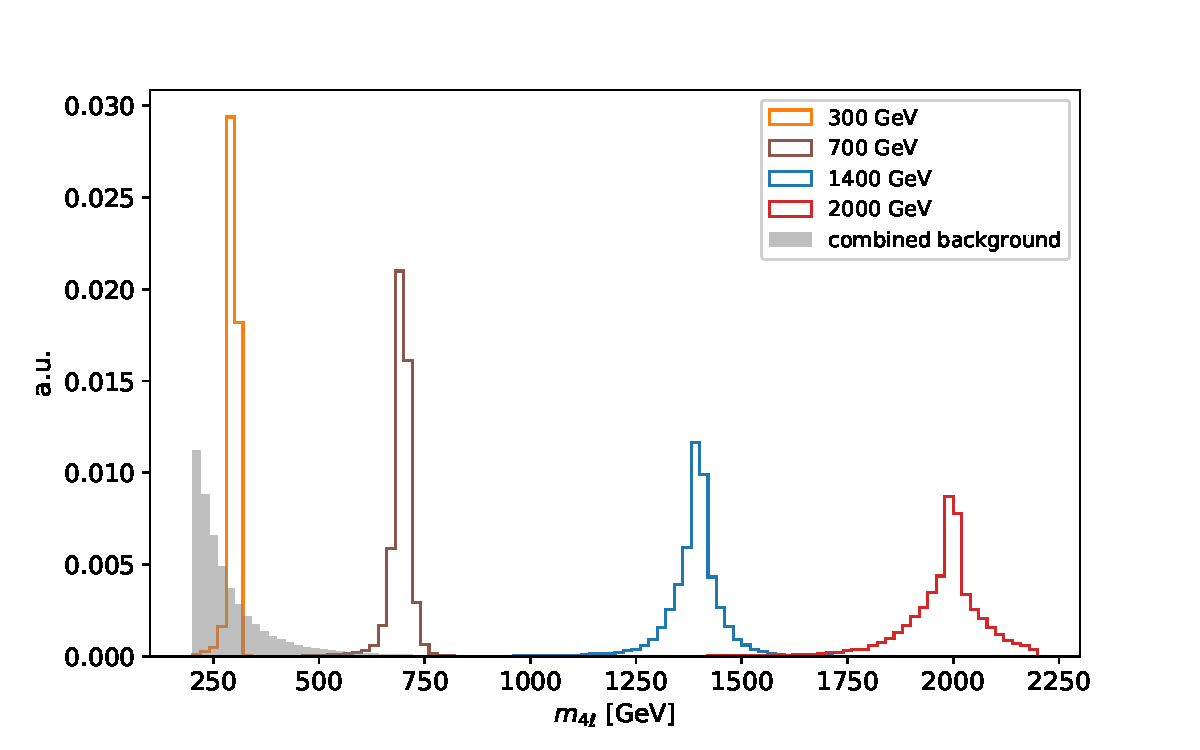
\includegraphics[width=0.24\textwidth]{figures/HMHZZ/selection/ggf_input/input_comparison_300_to_2000_5_score_m4l_unconstrained}}
%        \subfloat[]{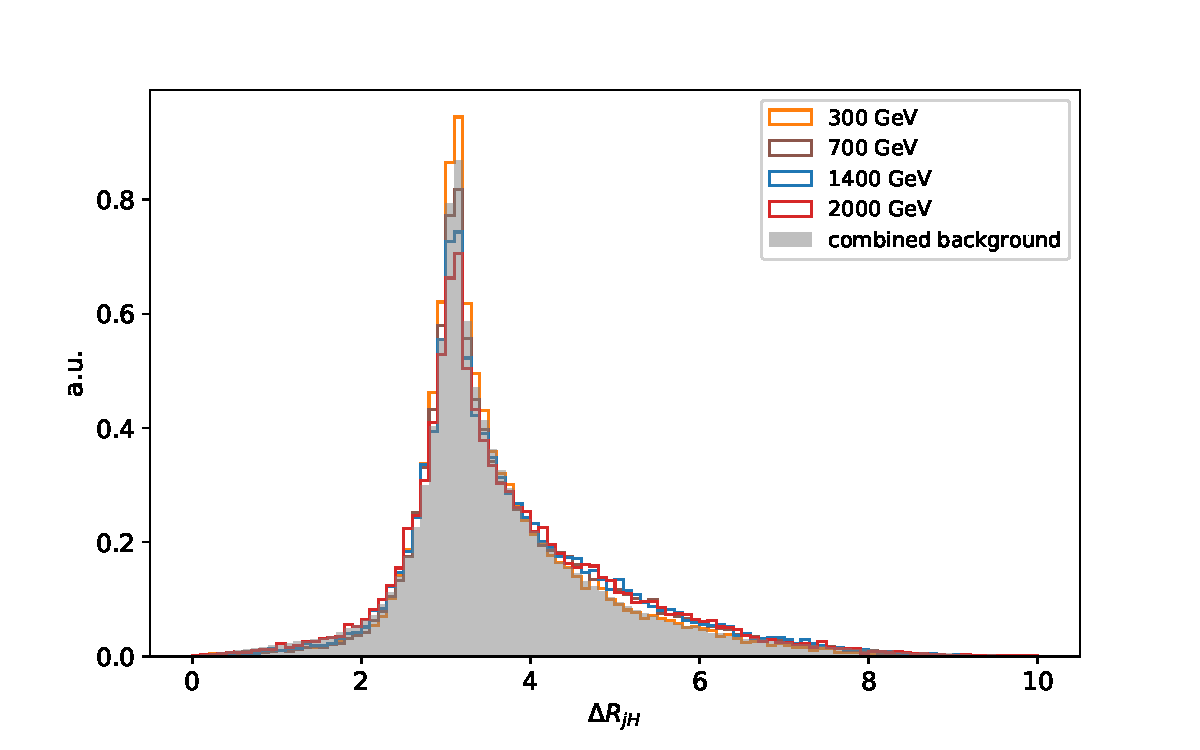
\includegraphics[width=0.24\textwidth]{figures/HMHZZ/selection/ggf_input/input_comparison_300_to_2000_6_score_dR_jH}}
%        \subfloat[]{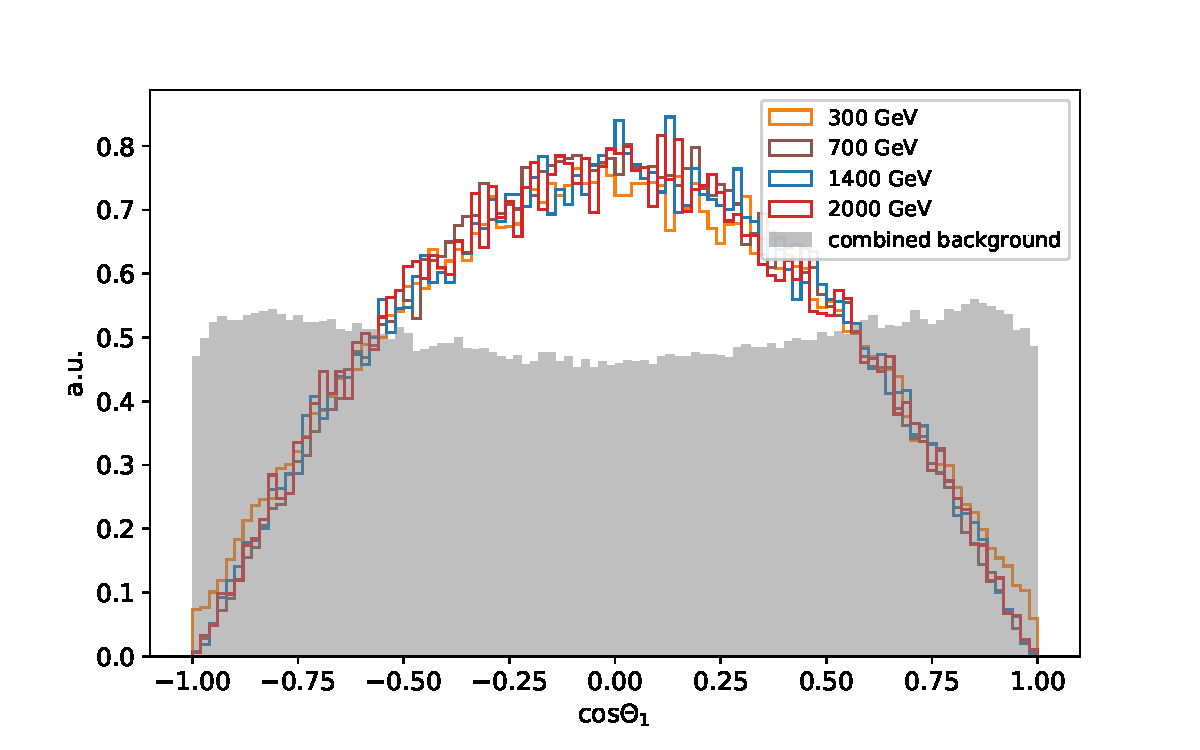
\includegraphics[width=0.24\textwidth]{figures/HMHZZ/selection/ggf_input/input_comparison_300_to_2000_7_score_cth1_unconstrained}}
%        \subfloat[]{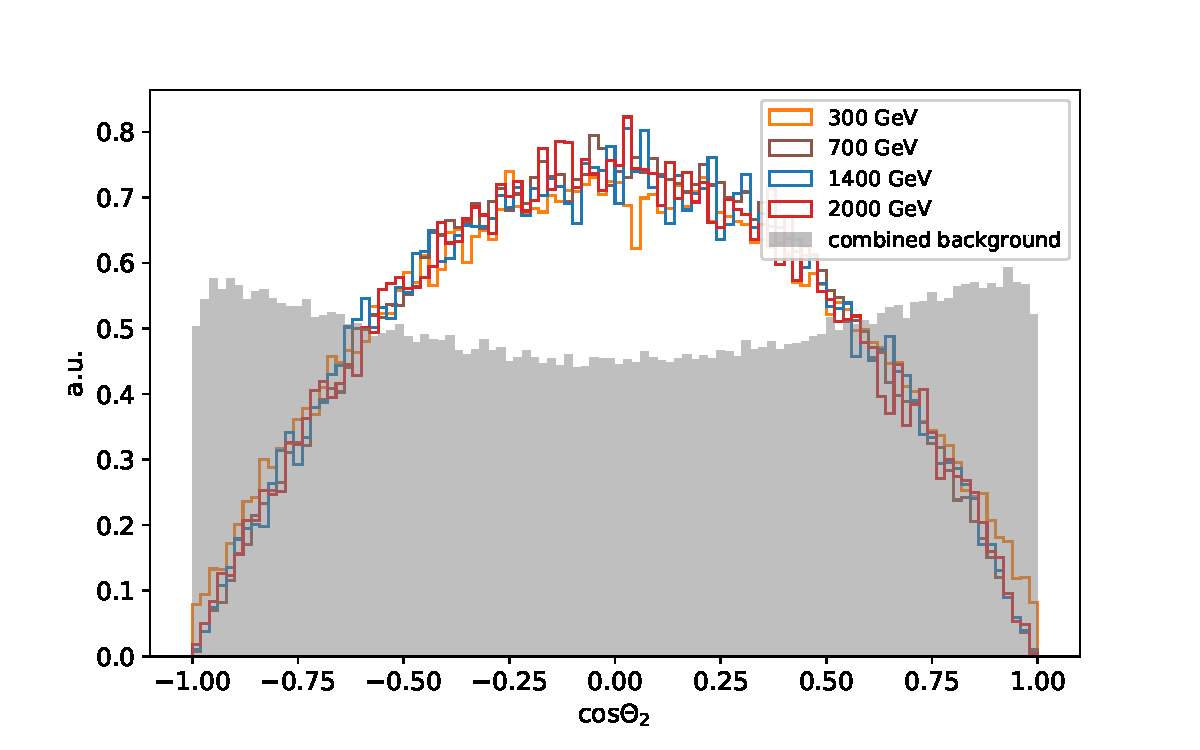
\includegraphics[width=0.24\textwidth]{figures/HMHZZ/selection/ggf_input/input_comparison_300_to_2000_8_score_cth2_unconstrained}}\\
%
%        \subfloat[]{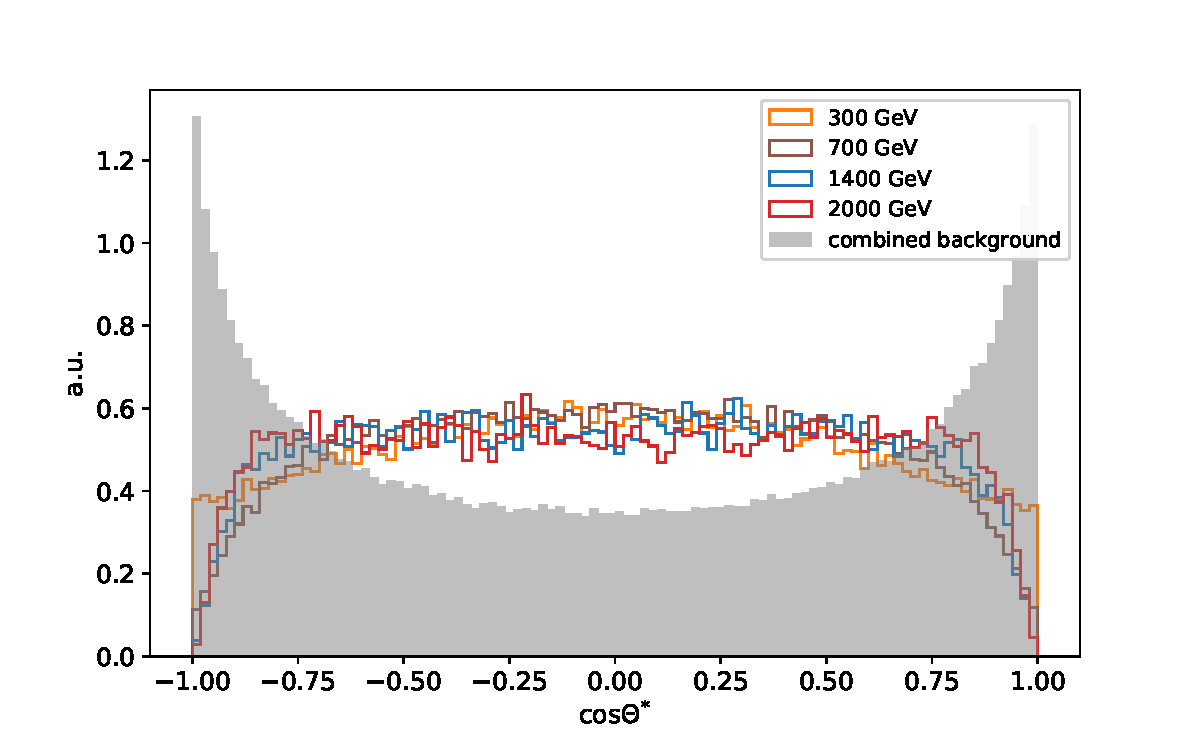
\includegraphics[width=0.24\textwidth]{figures/HMHZZ/selection/ggf_input/input_comparison_300_to_2000_9_score_cthstr_unconstrained}}
%        \subfloat[]{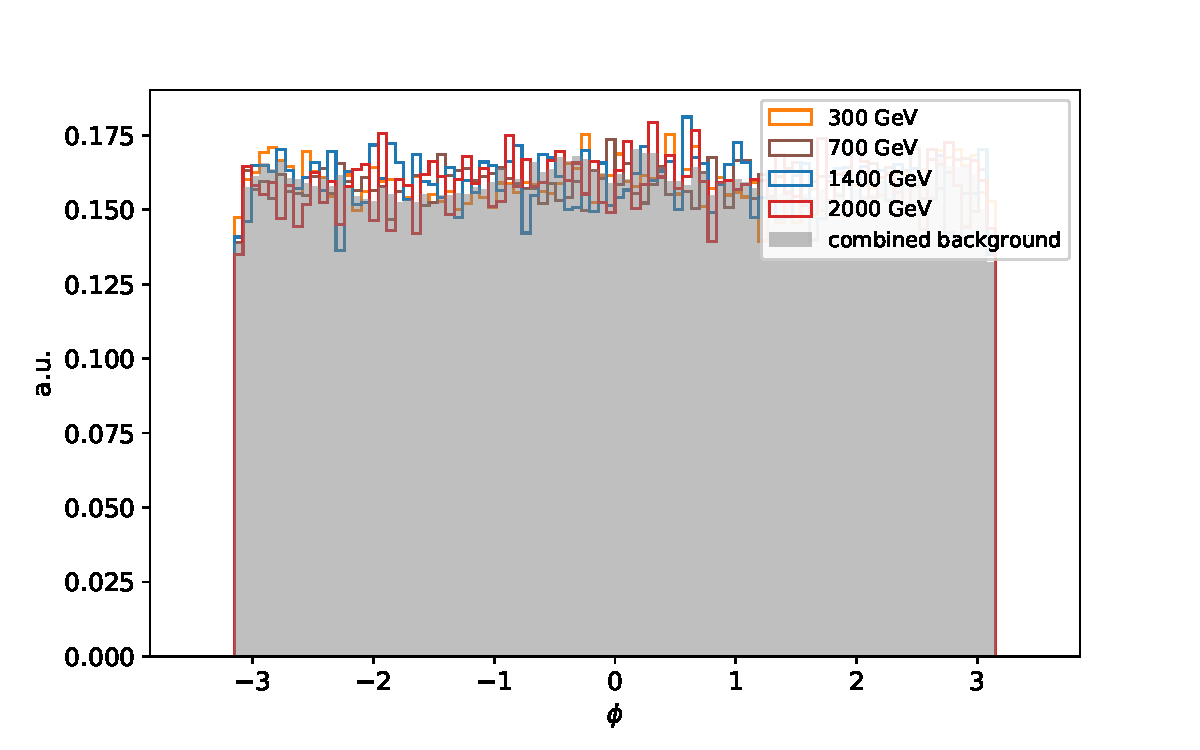
\includegraphics[width=0.24\textwidth]{figures/HMHZZ/selection/ggf_input/input_comparison_300_to_2000_10_score_phi_unconstrained}}
%        \subfloat[]{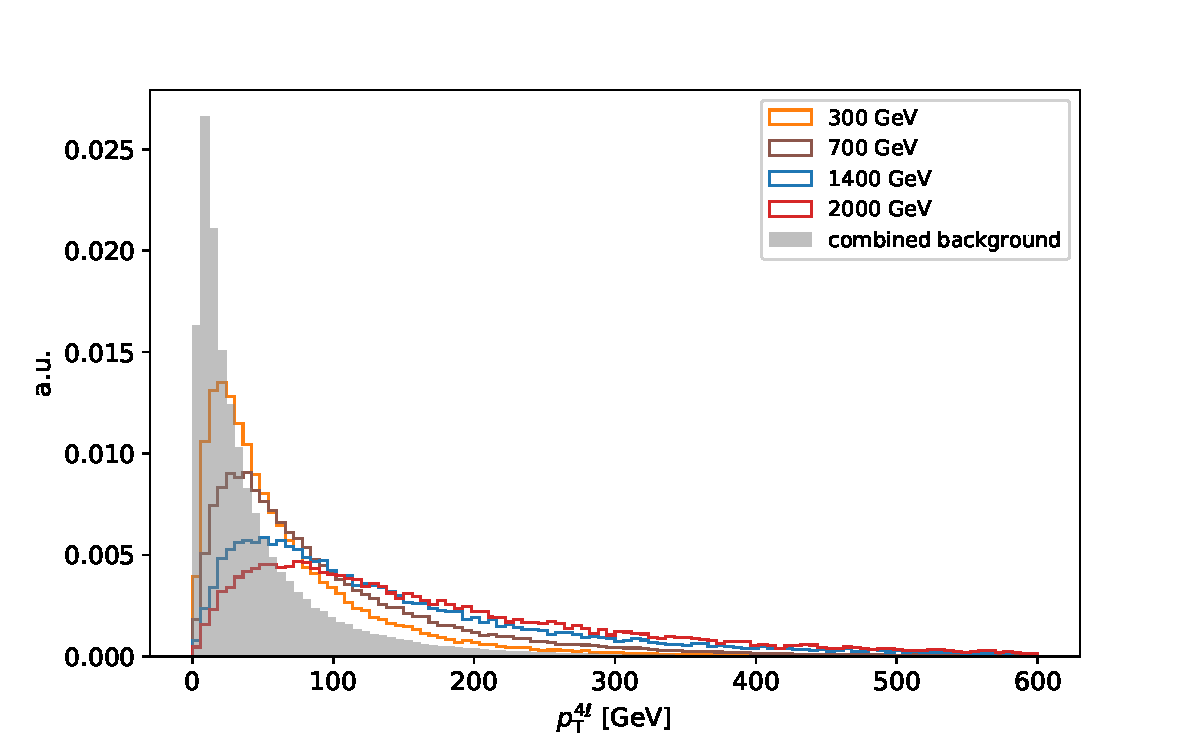
\includegraphics[width=0.24\textwidth]{figures/HMHZZ/selection/ggf_input/input_comparison_300_to_2000_11_score_pt4l_unconstrained}}
%        \subfloat[]{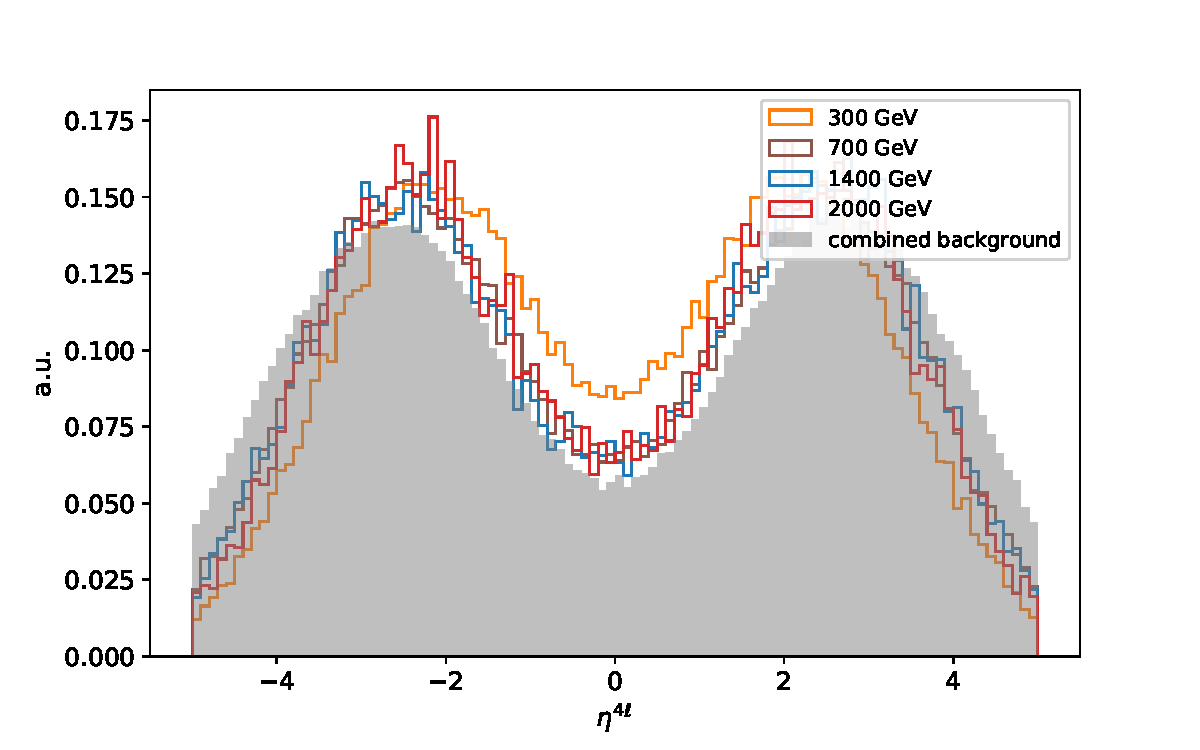
\includegraphics[width=0.24\textwidth]{figures/HMHZZ/selection/ggf_input/input_comparison_300_to_2000_12_score_eta4l_unconstrained}}\\
%
%        \subfloat[]{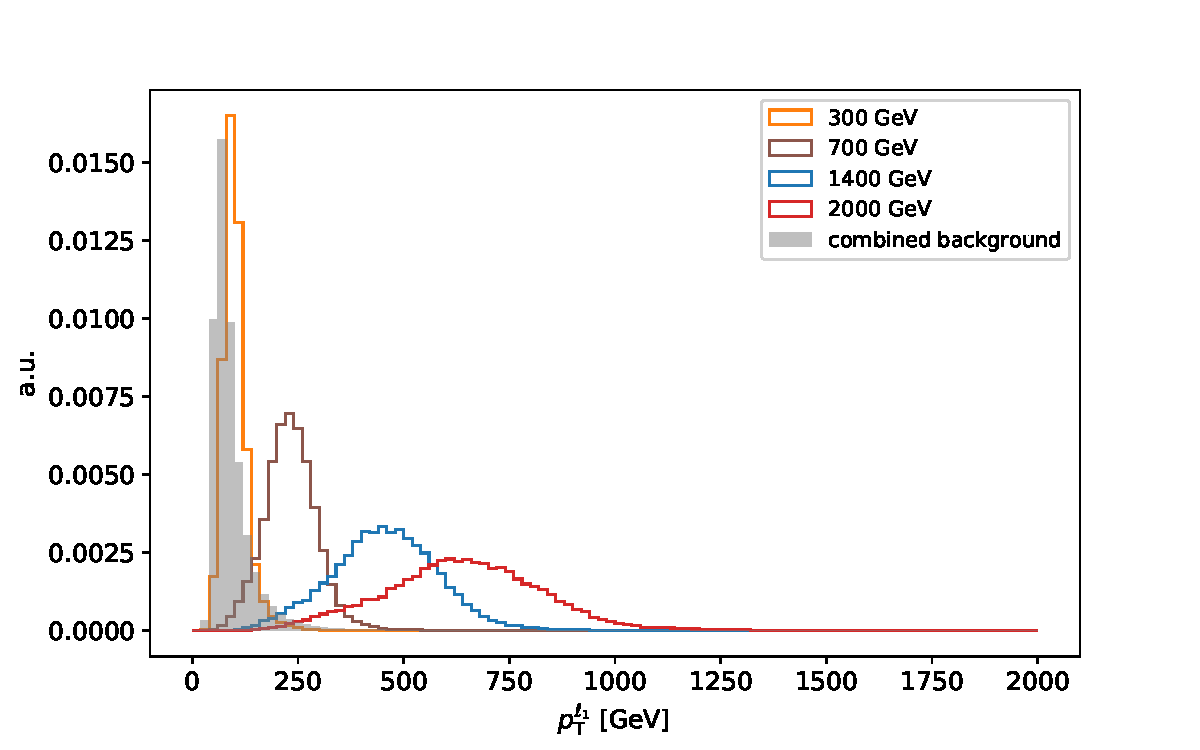
\includegraphics[width=0.24\textwidth]{figures/HMHZZ/selection/ggf_input/input_comparison_300_to_2000_15_score_lep_1_pt}}
%        \subfloat[]{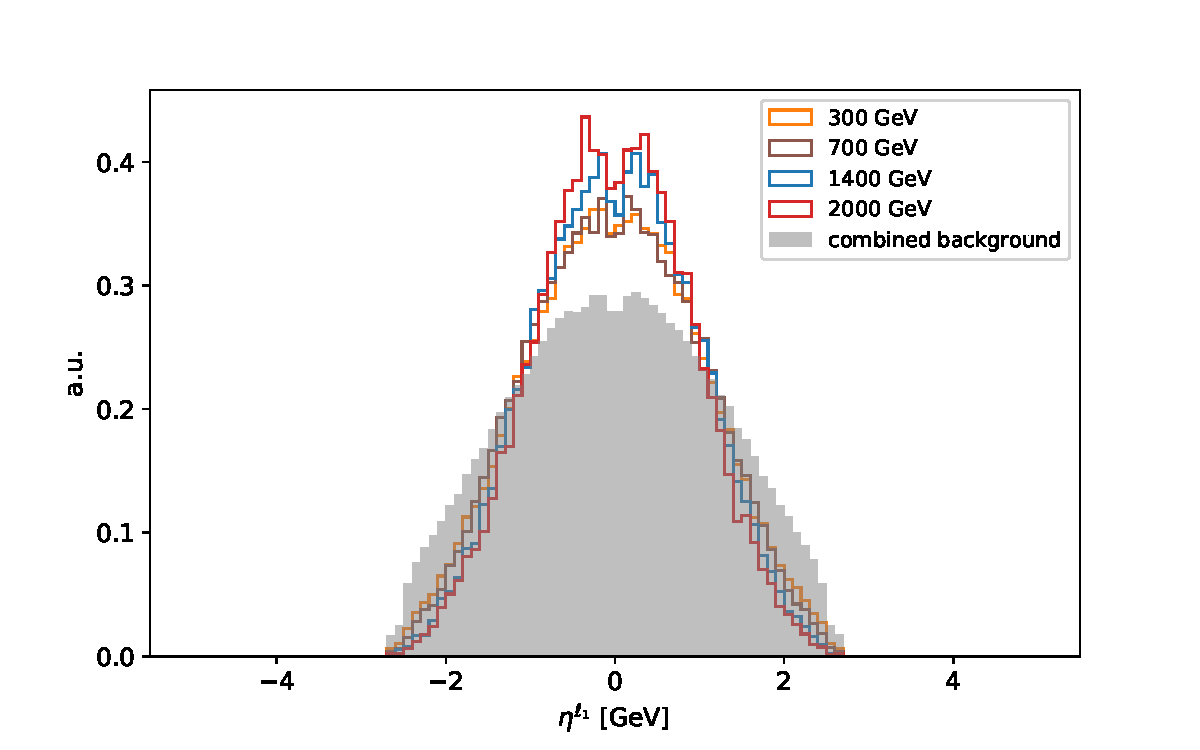
\includegraphics[width=0.24\textwidth]{figures/HMHZZ/selection/ggf_input/input_comparison_300_to_2000_16_score_lep_1_eta}}
%        \subfloat[]{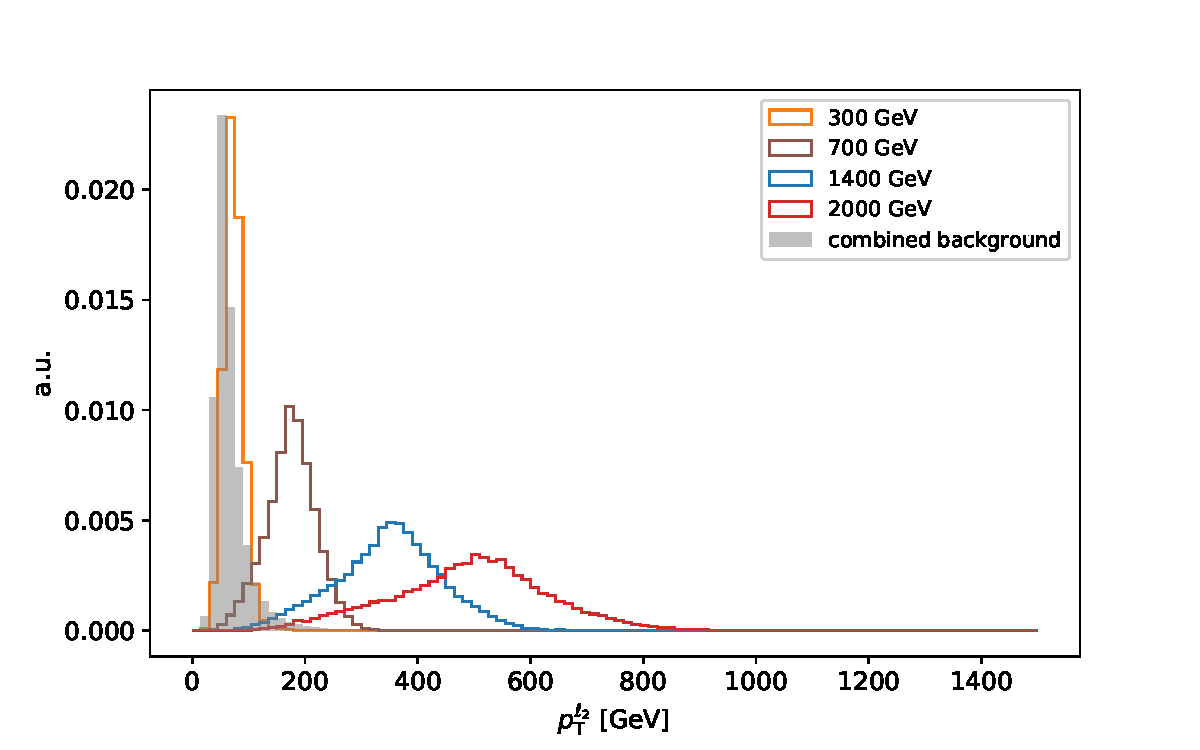
\includegraphics[width=0.24\textwidth]{figures/HMHZZ/selection/ggf_input/input_comparison_300_to_2000_17_score_lep_2_pt}}
%        \subfloat[]{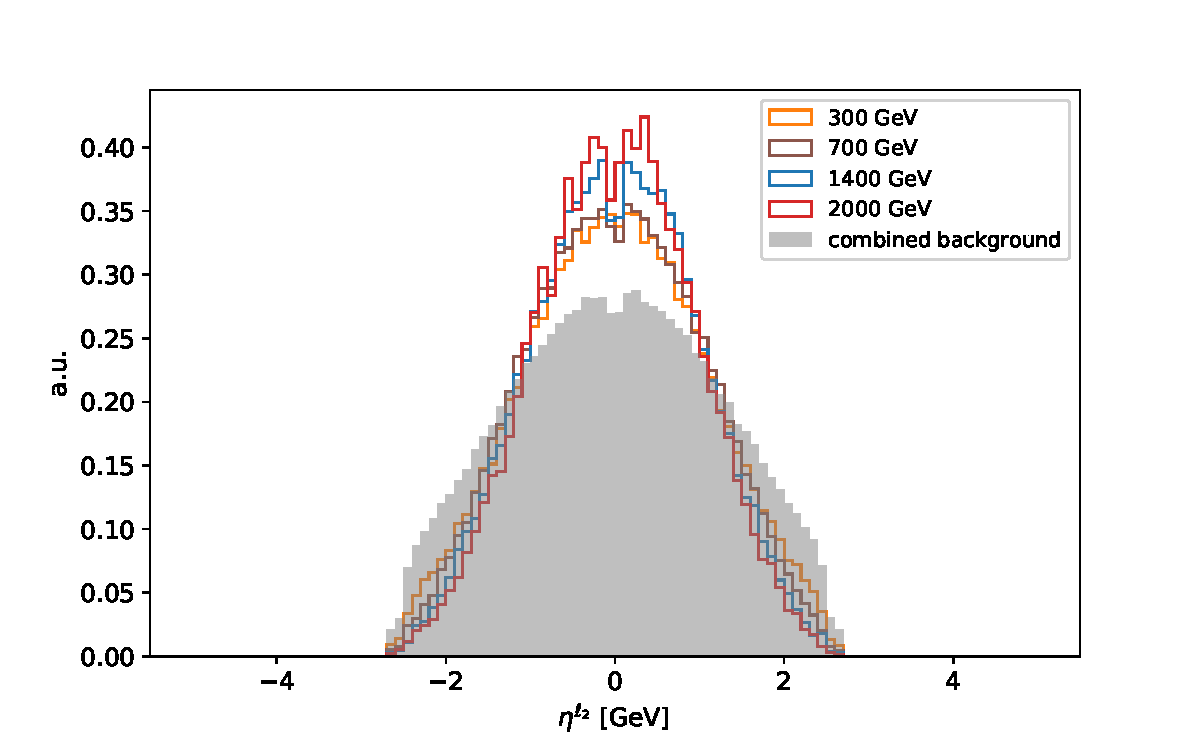
\includegraphics[width=0.24\textwidth]{figures/HMHZZ/selection/ggf_input/input_comparison_300_to_2000_18_score_lep_2_eta}}\\
%
%        \subfloat[]{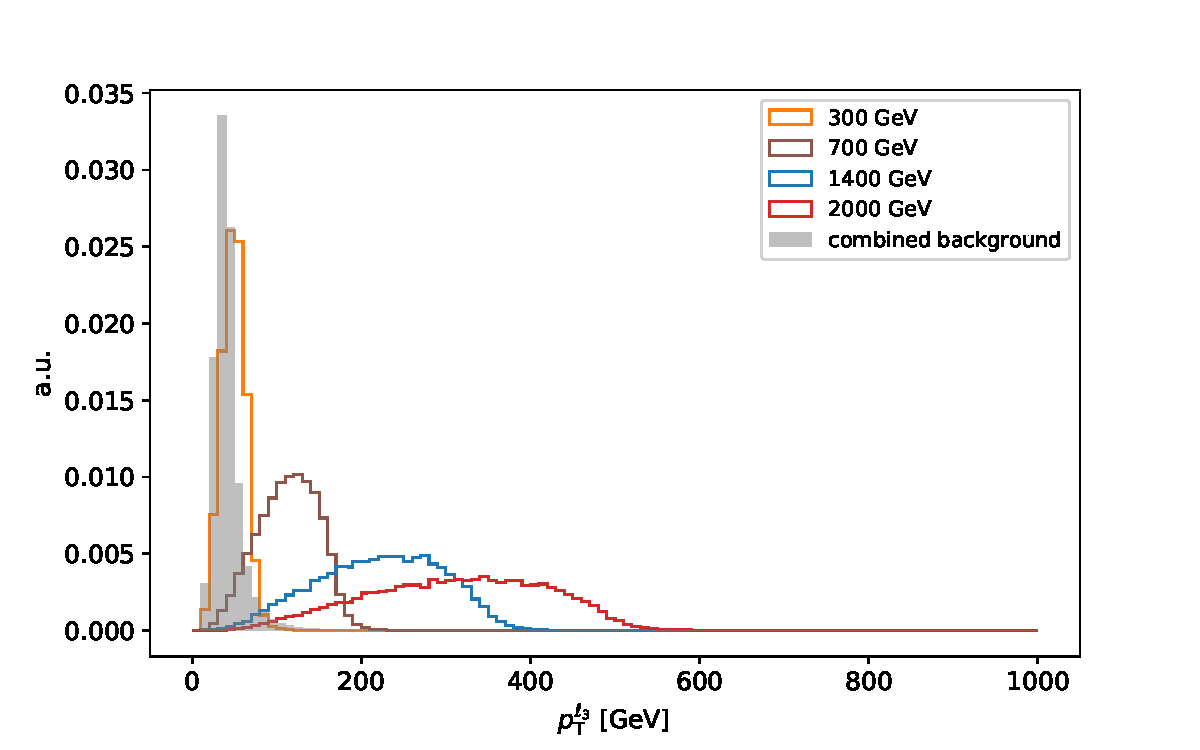
\includegraphics[width=0.24\textwidth]{figures/HMHZZ/selection/ggf_input/input_comparison_300_to_2000_19_score_lep_3_pt}}
%        \subfloat[]{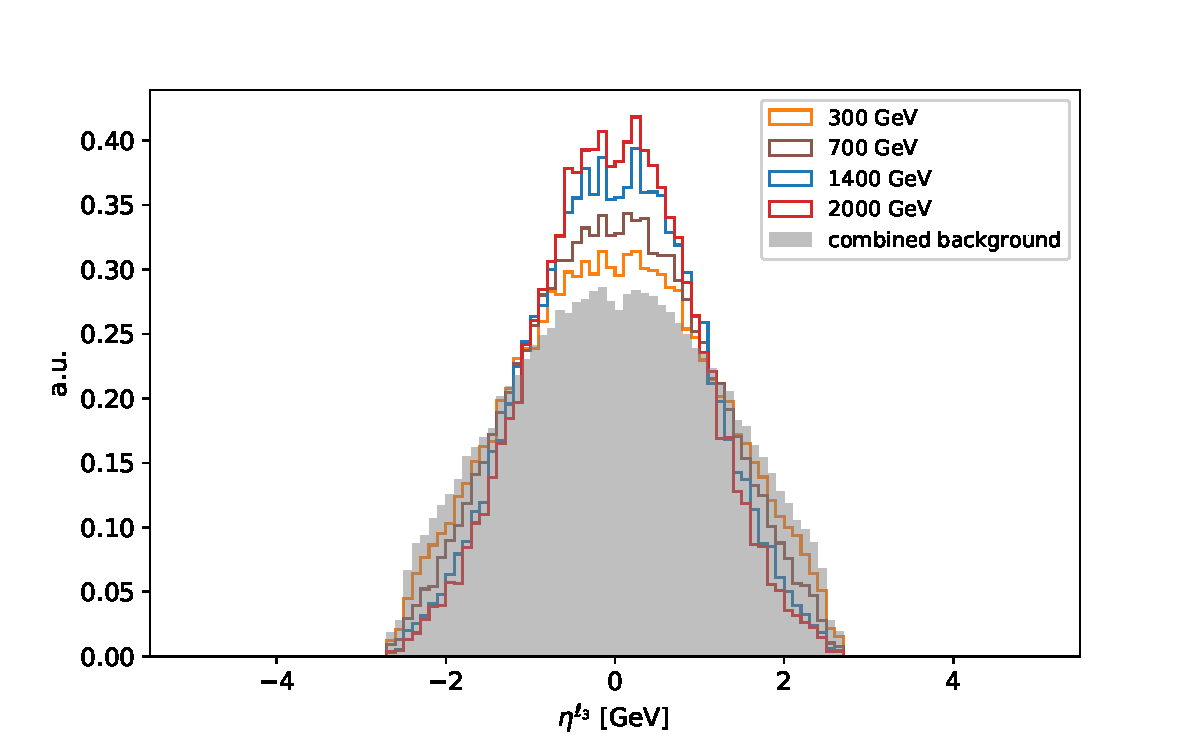
\includegraphics[width=0.24\textwidth]{figures/HMHZZ/selection/ggf_input/input_comparison_300_to_2000_20_score_lep_3_eta}}
%        \subfloat[]{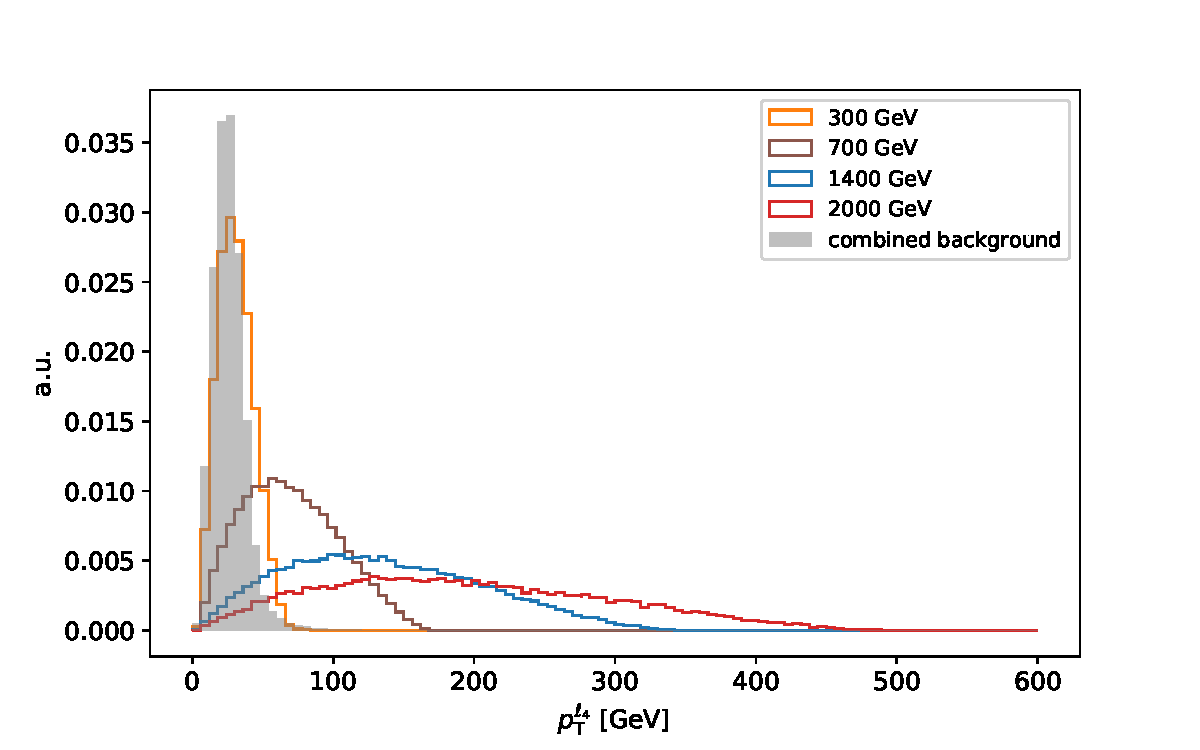
\includegraphics[width=0.24\textwidth]{figures/HMHZZ/selection/ggf_input/input_comparison_300_to_2000_21_score_lep_4_pt}}
%        \subfloat[]{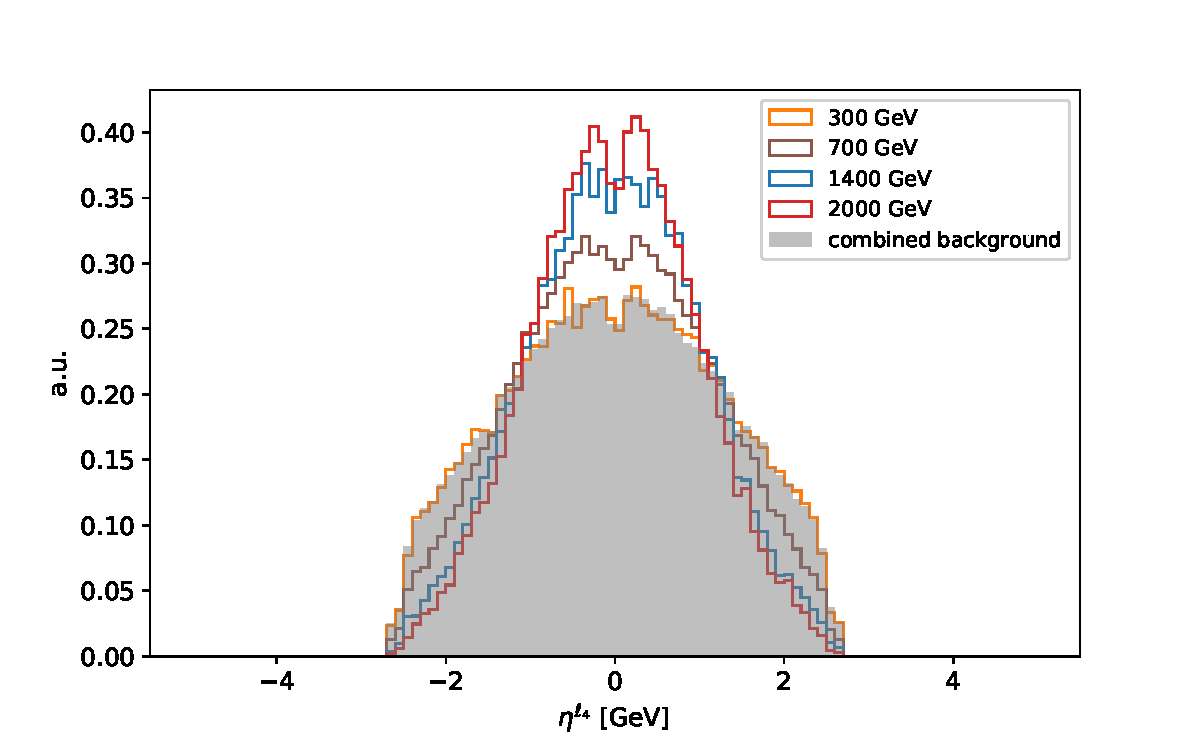
\includegraphics[width=0.24\textwidth]{figures/HMHZZ/selection/ggf_input/input_comparison_300_to_2000_22_score_lep_4_eta}}\\
%
%        \caption{Distributions of input features as listed in table~\ref{tab:dnn_features_ggf} for the ggF network of signals at mass points of 300, 700, 1400, 2000~\gev (coloured) and the background (grey). Events with any jet multiplicity are shown, as this model is evaluated in both $N_\mathrm{jets}\geq2$ and $N_\mathrm{jets}<2$.}
%        \label{fig:dnn_ggf_distribution}
%\end{figure}

\textbf{Evaluation of models} 

Figure~\ref{fig:dnn_output_score} shows the output of ``ggF-classifier'' and ``VBF-classifier'' for data, SM backgrounds and an example signal at 600~\gev.
The ggF and VBF signals cross section are set to be 100 times of their observed upper limit described in section~\ref{sec:hmhzz_spin0nwa} for ggF output
and 30 times of the observed upper limit for VBF output for best visibility.

\begin{figure}[htbp]
        \subfloat[]{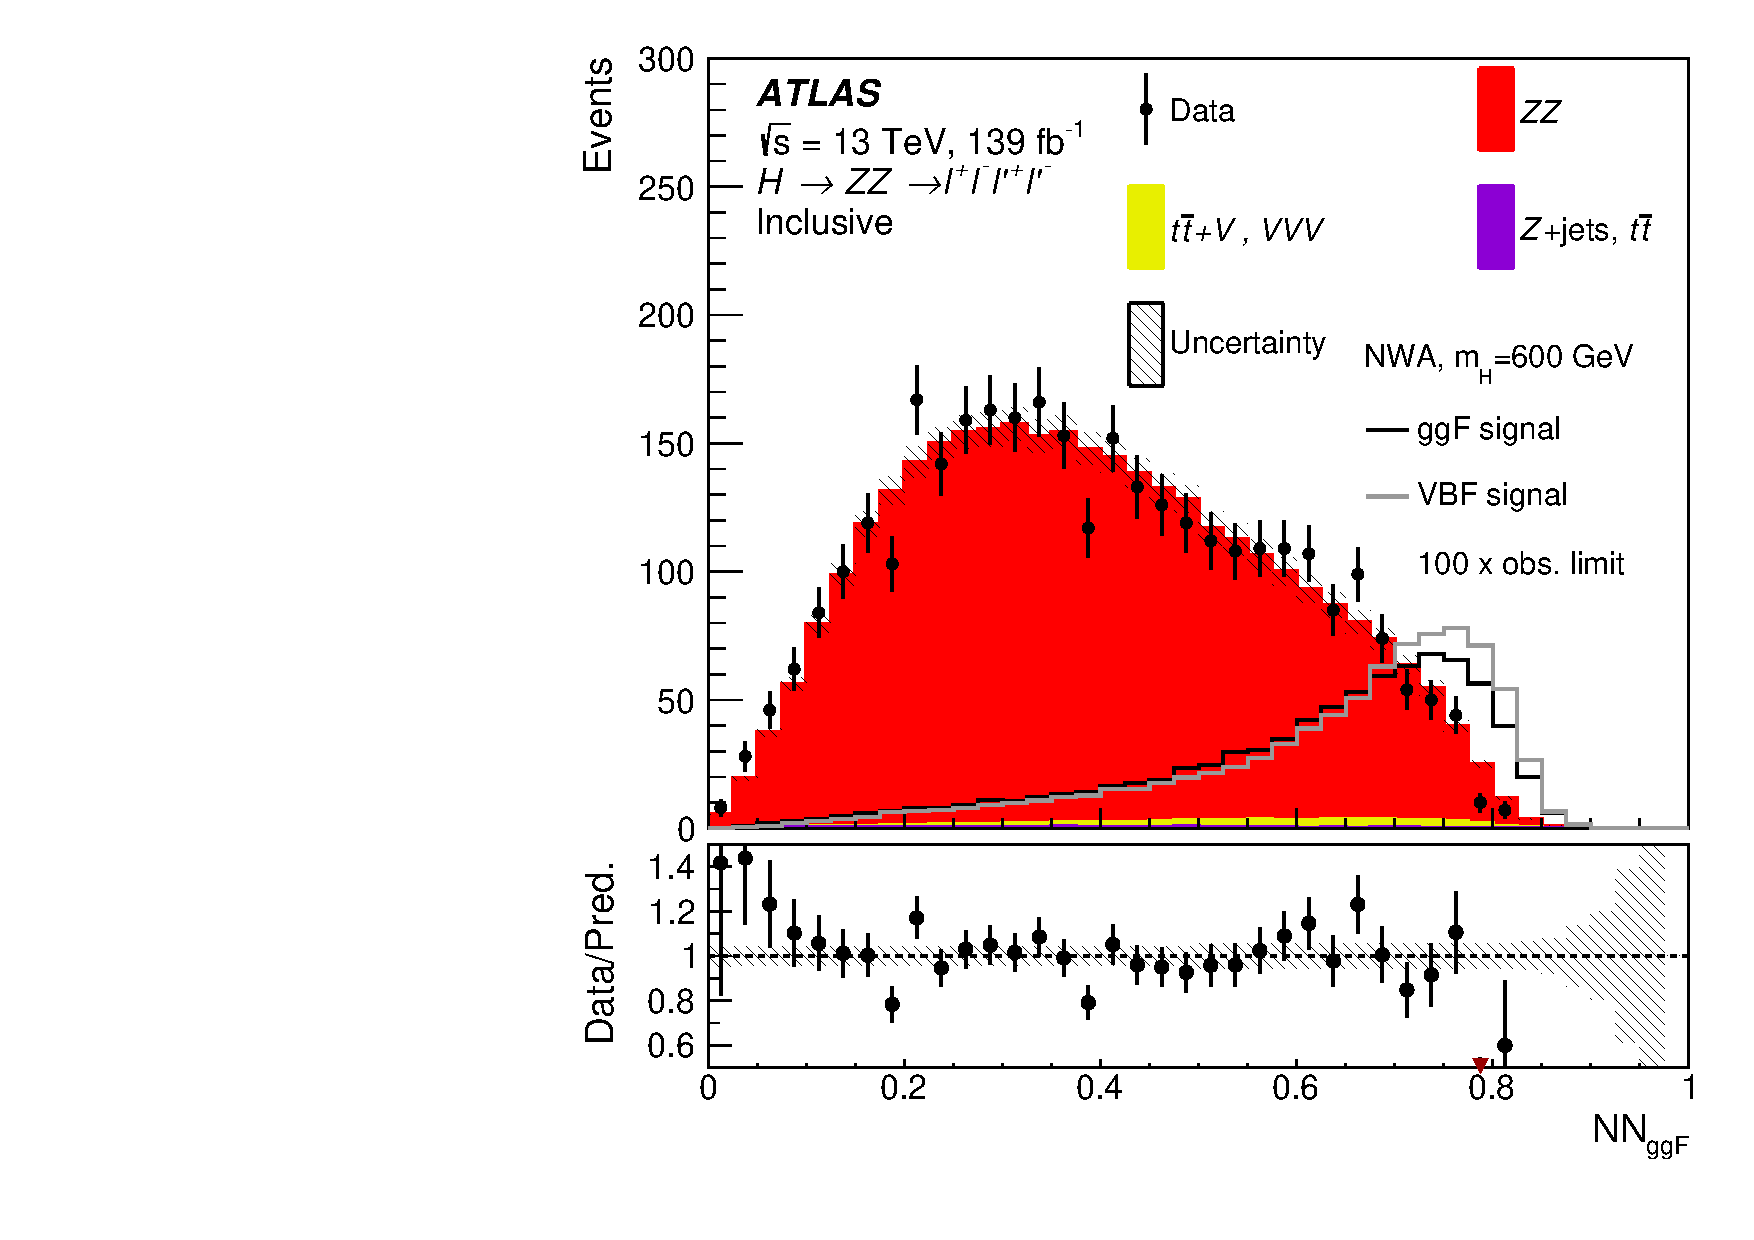
\includegraphics[width=0.48\textwidth]{figures/HMHZZ/results/4l_DNN_scores_ggF_incl.pdf}}
        \subfloat[]{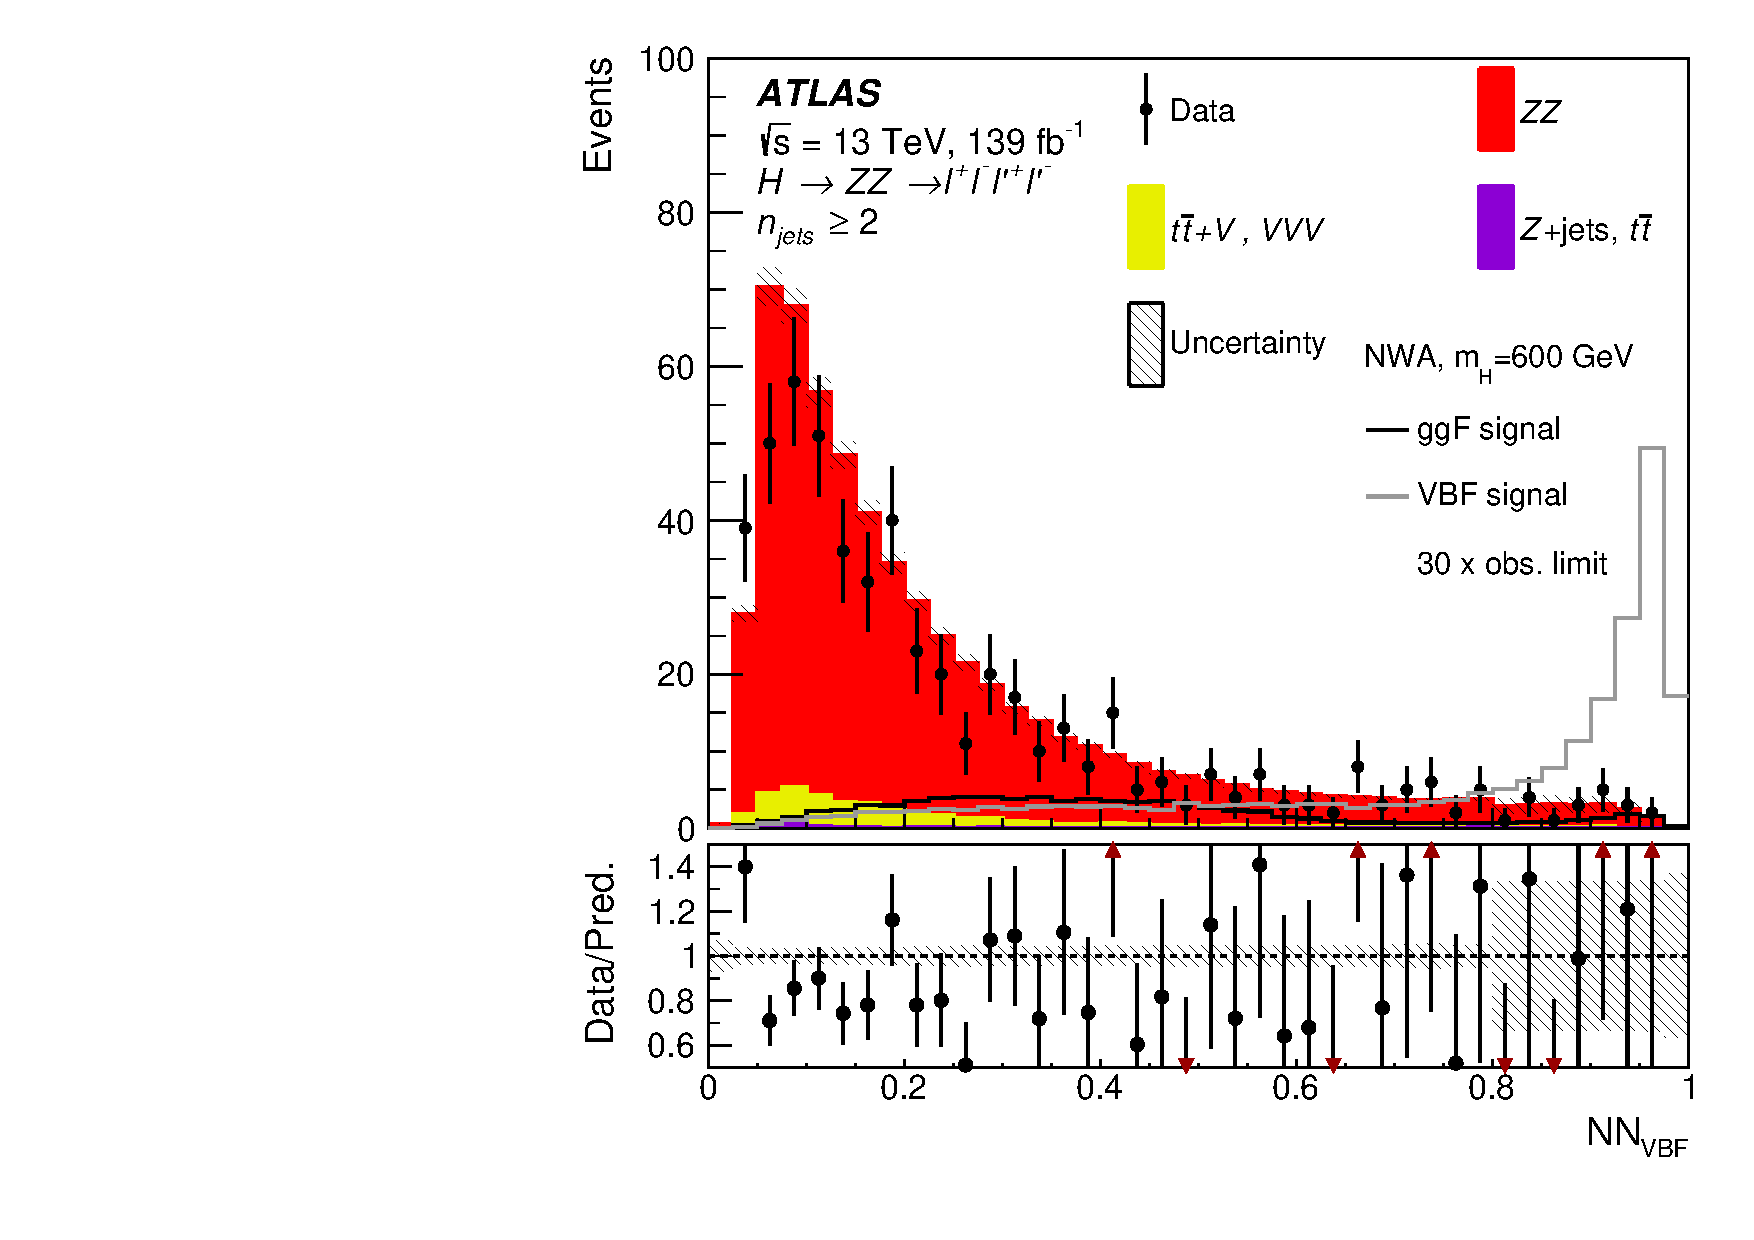
\includegraphics[width=0.48\textwidth]{figures/HMHZZ/results/4l_DNN_scores_VBF_incl.pdf}}
        \centering
        \caption{The output score of ``ggF-classifier'' (a) and  ``VBF-classifer'' (b) with the events passing the common event selections  
        for the data, the SM backgrounds and an example of a NWA signal with a mass of $600~\gev{}$.
        For the ``VBF-classifier'', an additional requirement of at least two jets in the event is applied.
        The signals cross section are set to 100 times of the observed limit for the ``ggF-classifier'' 
        and 30 times of the observed limit for the ``VBF~-classifer''.
        The $ZZ$ backgrounds are scaled by the normalisation factors shown in Table~\ref{tab:muZZ_bonly_dnn}.
        The lower panels show the ratio of data to prediction.
        Statistical and experimental systematic uncertainties are included.}
        \label{fig:dnn_output_score}
\end{figure}

Then the optimal cut at output score from each classifier is chosen based on an overall good performance of classifier to have a large significance improvement while retaining a high signal efficiency.
Figure~\ref{fig:dnn_significance} shows the significance improvements of MVA-based cuts when comparing with cut-based one at different VBF (left) and ggF (right) mass samples,
where the significance is calculated from an asymptotic approximation~\cite{2008NIMPA.595..480C}:
\begin{equation}
Z = \sqrt{2\left(n\ln \left[ \frac{nb+\sigma_b^2}{b^2+n\sigma_b^2}\right]
        - \frac{b^2}{\sigma_b^2}\ln\left[1+\frac{\sigma_b^2(n-b)}{b(b+\sigma_b^2)}\right]\right)}
\end{equation}
where n denotes to the sum of expected signal and background, b is the background, and $\sigma_b$ is the uncertainty of background.
Cut at 0.5 (0.8) for VBF (ggF) classifier is chosen as shown in solid lines.

\begin{figure}[htbp]
        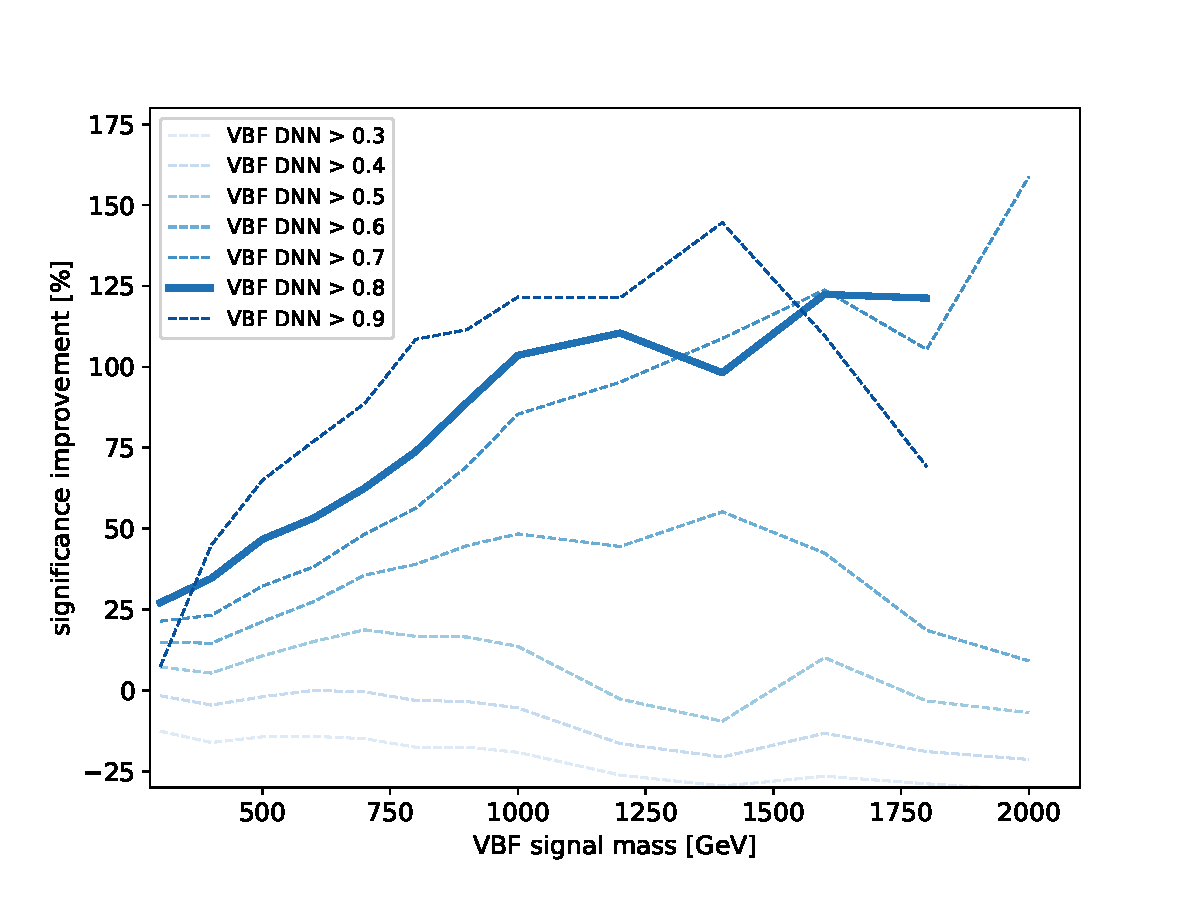
\includegraphics[width=0.48\textwidth]{figures/HMHZZ/selection/VBF_significance_improvement.pdf}
        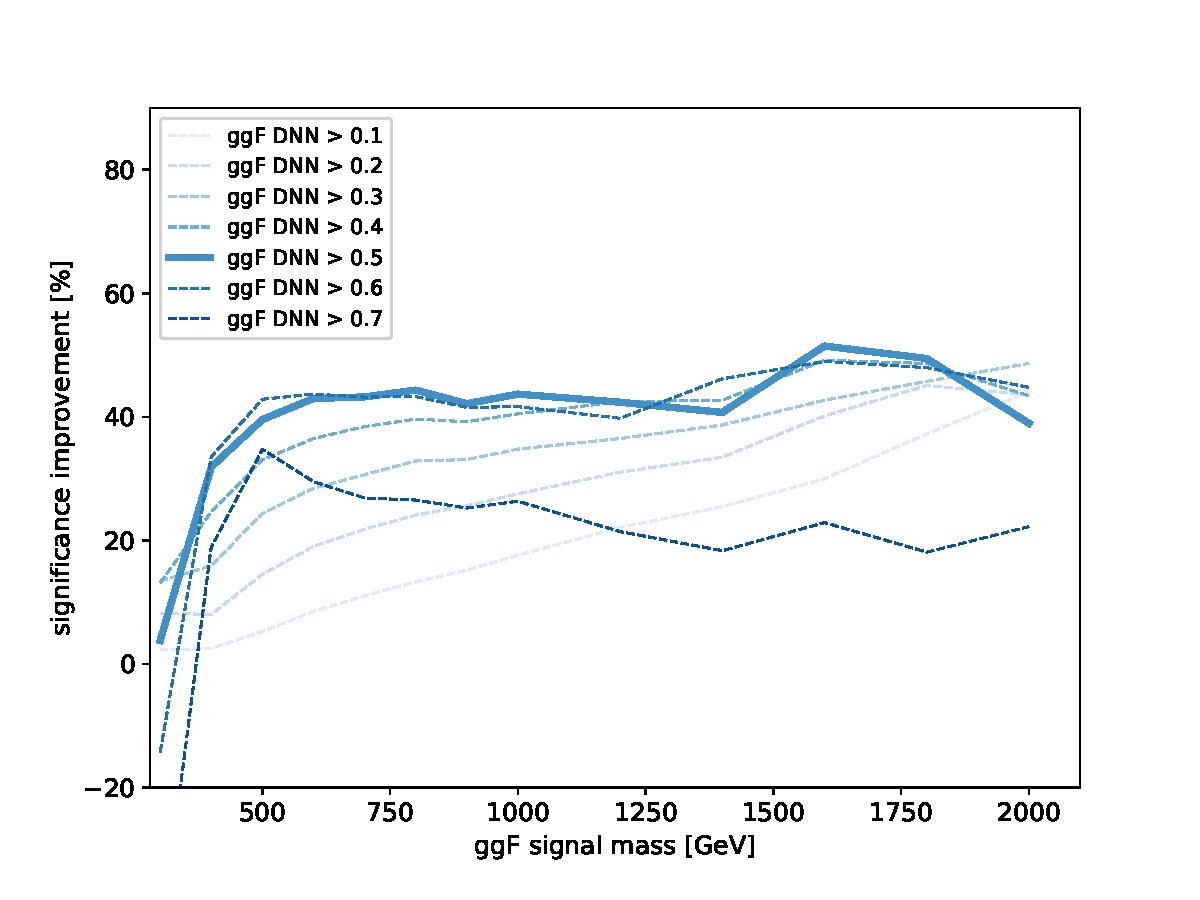
\includegraphics[width=0.48\textwidth]{figures/HMHZZ/selection/ggf_significance_improvement.pdf}
        \centering
        \caption{Significance improvements of the MVA-based over the cut-based categorization of the VBF (ggF) category for VBF (ggF) signal samples from 300 to 2000~\gev~ for seven different cuts on the VBF (ggF) output score. 
	The optimal cut of 0.8 (0.5) for VBF (ggF) score is chosen as the solid line, while other alternative cuts are plotted with dashed lines. 
	For VBF category, results at 2000~\gev~ for cuts of 0.8 and 0.9 are missing due to a lack of background events passing this tight selection.}
        \label{fig:dnn_significance}
\end{figure}

Then the events passing VBF classifier are categorized into VBF-MVA-enriched category.
Otherwise, the events failing VBF classifier but passing ggF classifier are categorized into ggF-MVA-high category, which is further split into 3 channels based on their lepton flavor.
All remaining events are sorted into one additional ggF-MVA-low category.
Thus there are five categories defined in MVA-based categorization.
In summary, cuts applied in categorization are defined as follow, and these different phase spaces are also illustrated in figure~\ref{fig:hmhzz_dnncate}.

\begin{itemize}
	\item VBF-MVA-enriched category: Events have at least two selected jets ($\Njets \geq 2$), and with \DNNVBF > 0.8;
	\item ggF-MVA-high categories: $(\Njets \geq 2 \:\&\&\: \DNNVBF \leq 0.8 \:\&\&\: \DNNggF > 0.5) \:||\: (\Njets < 2 \:\&\&\: \DNNggF > 0.5)$; 
	\item ggF-MVA-low category: All remaining events that fail VBF and ggF cuts mentioned above.
\end{itemize}

\begin{figure}[h]
\centering
\subfloat[]{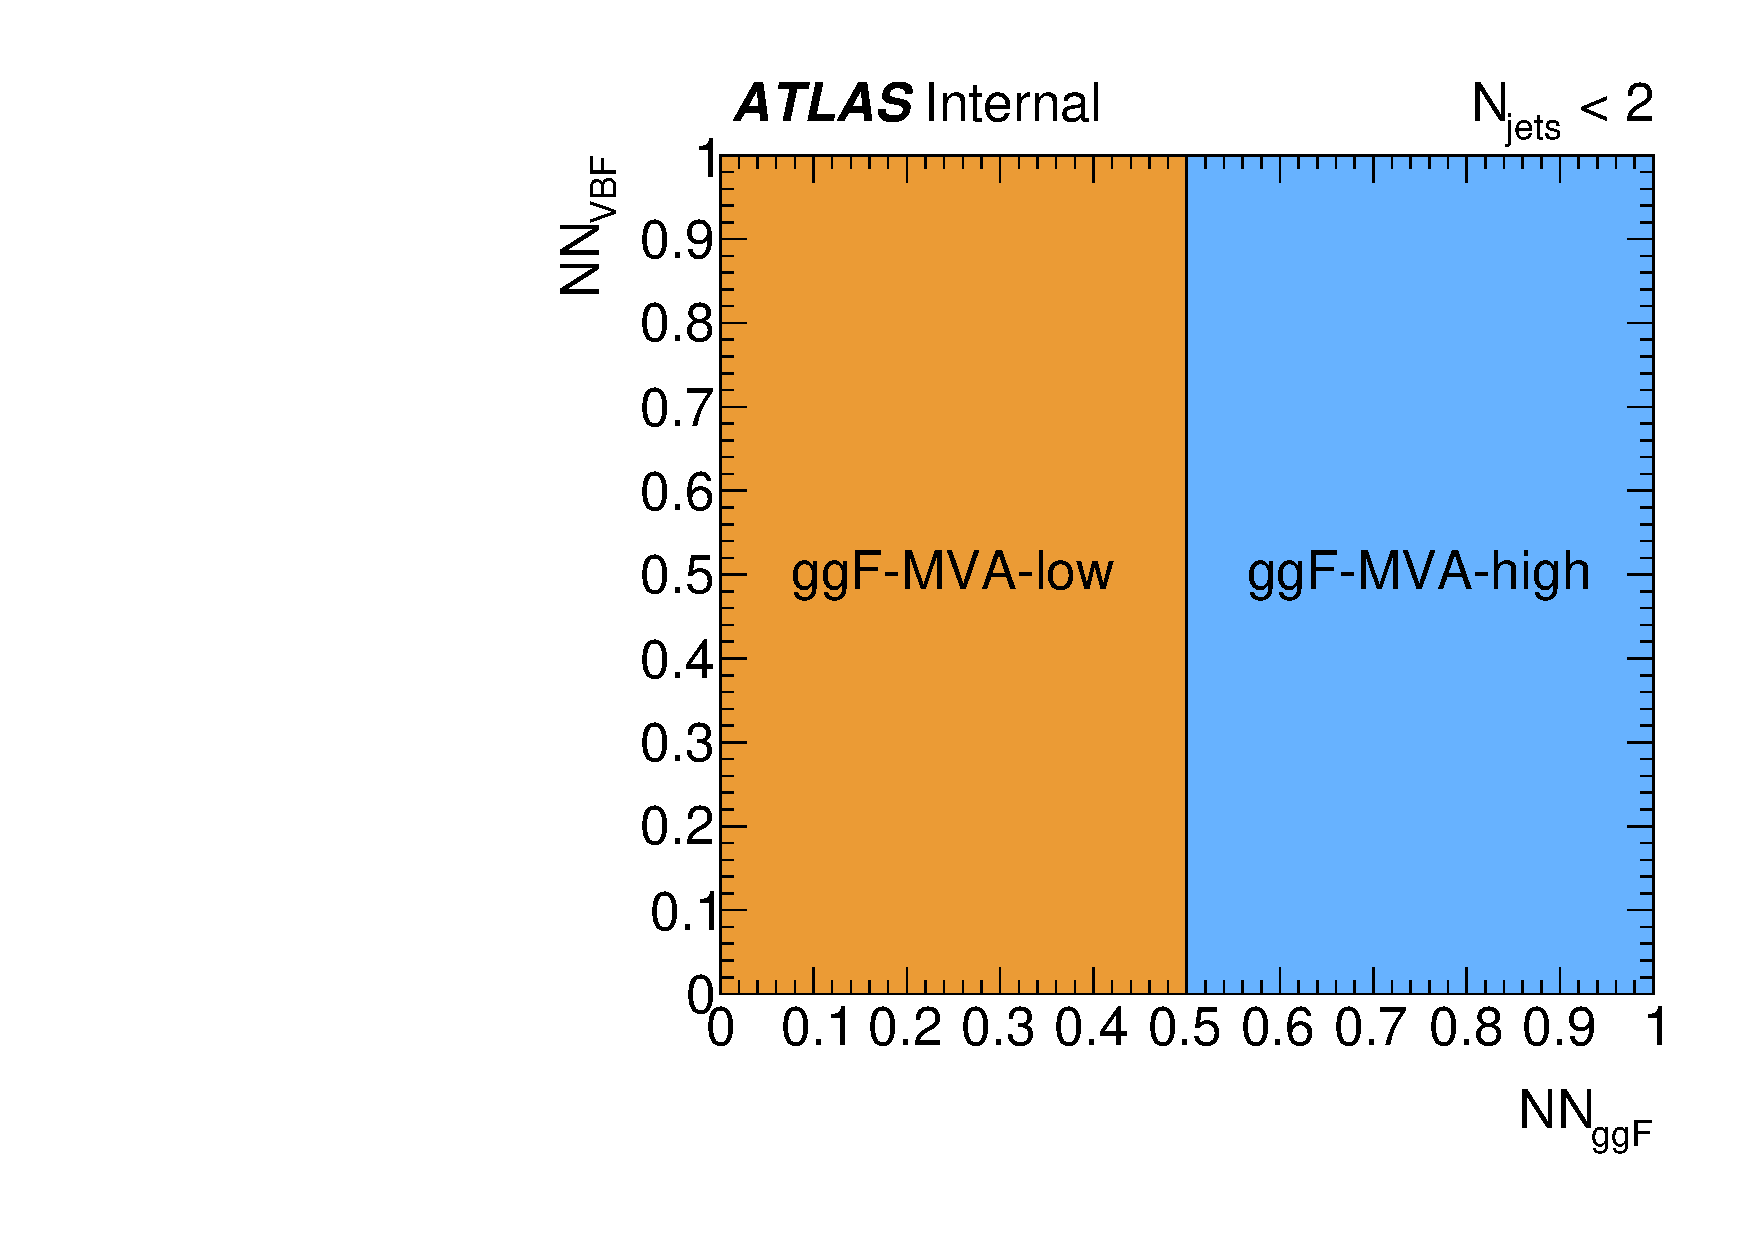
\includegraphics[width=0.43\textwidth]{figures/HMHZZ/selection/classifier_diagram_c1_njets_lt2.pdf}}
\subfloat[]{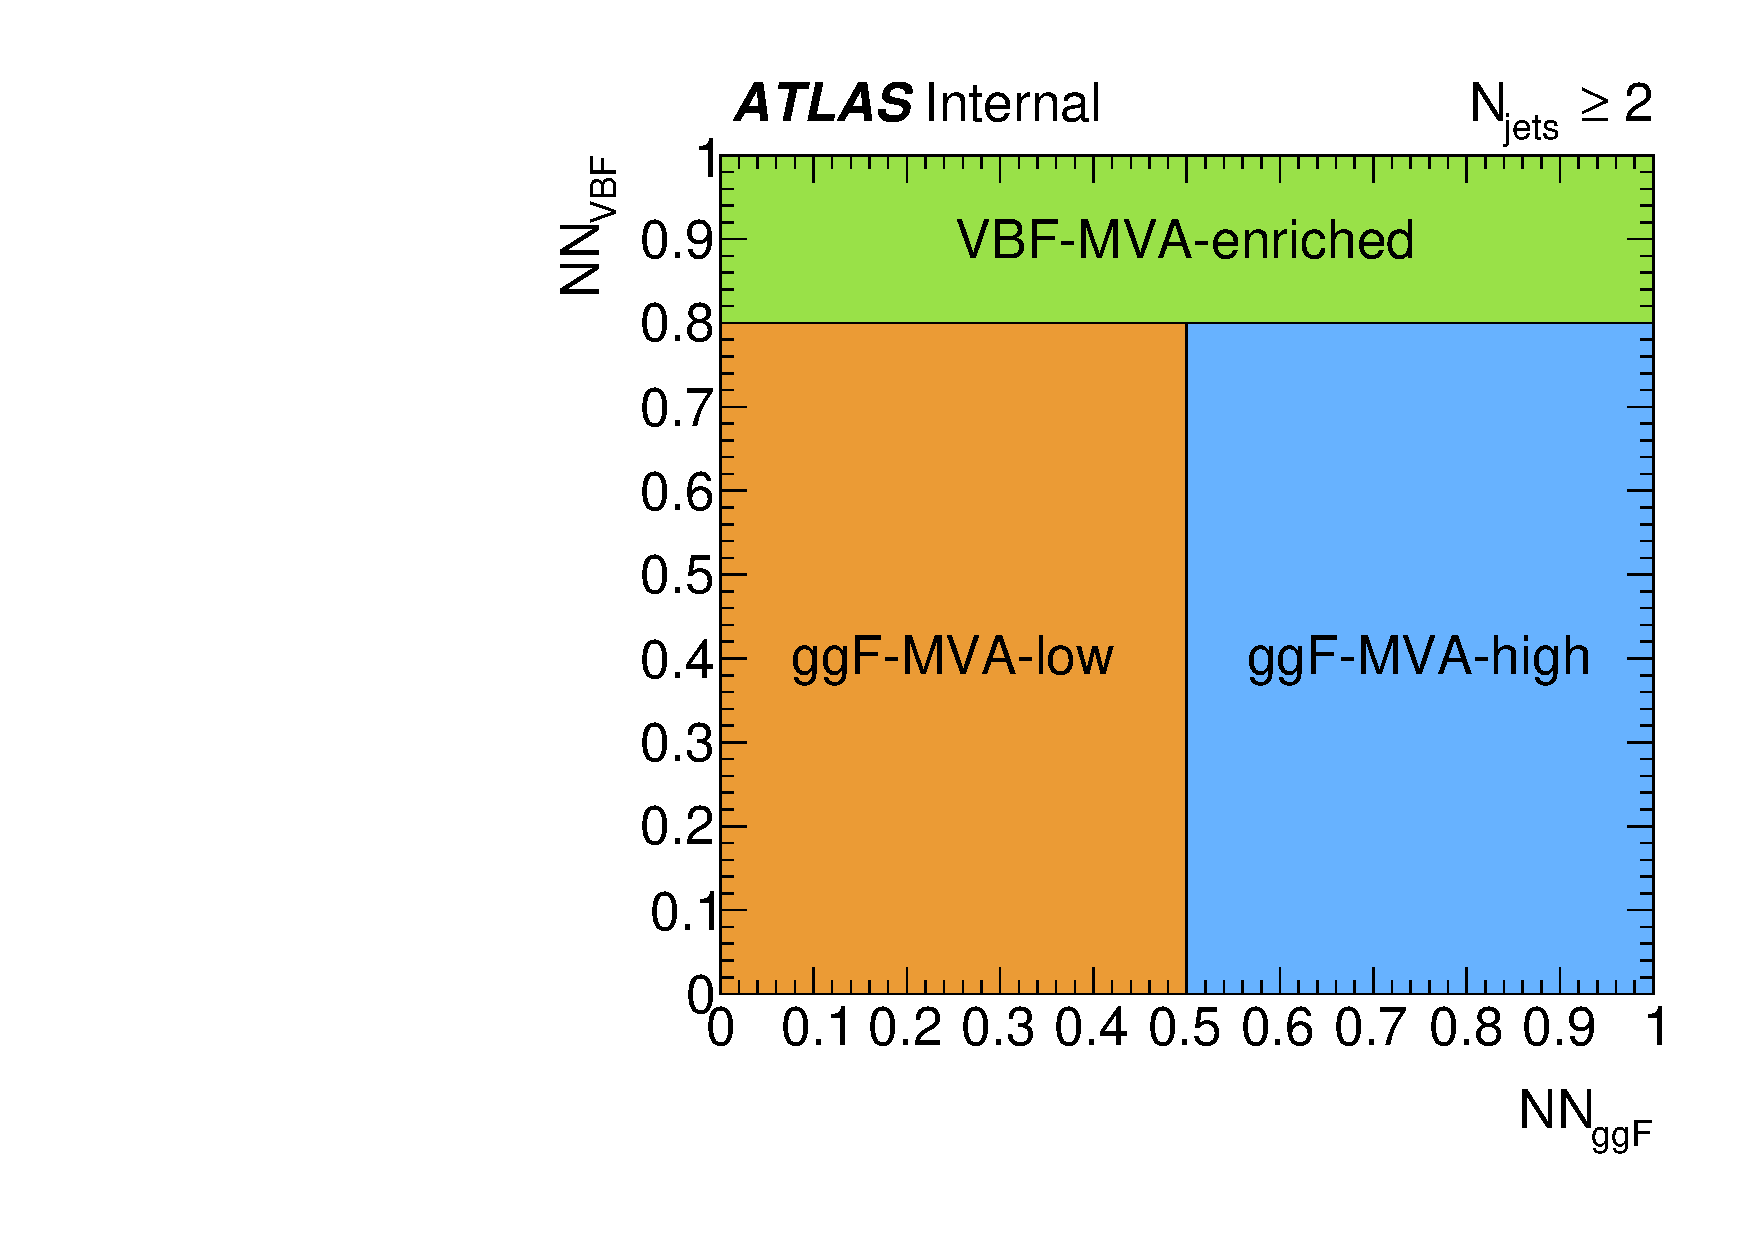
\includegraphics[width=0.43\textwidth]{figures/HMHZZ/selection/classifier_diagram_c1_njets_gt2.pdf}}\\
\caption{Illustration of the MVA-based VBF and ggF event classification for events with (a) $\Njets < 2$ and (b) $\Njets \geq 2$.}
\label{fig:hmhzz_dnncate}
\end{figure}

\subsection{Signal acceptance} 
\label{sec:hmhzz_signal_acc}
The signal acceptance is defined as the ratio of events passing all analysis selection in each category to the total number of simulated events in whole phase space.
In denominator, the events with $\tau$ final states are not taken into account.
And the contribution of $\tau$-lepton decay to electrons and muons final states is found to be negligible.

Figure~\ref{fig:hmhzz_acc_dnn} and ~\ref{fig:hmhzz_acc_cut} show the acceptance of NWA signals in DNN- and Cut- based categorization, estimated by merging the three signal MC campaigns, mc16a, mc16d and mc16e.
A 3-rd order polynomial fit is applied for each category.

\begin{figure}[h]
\centering
\subfloat[]{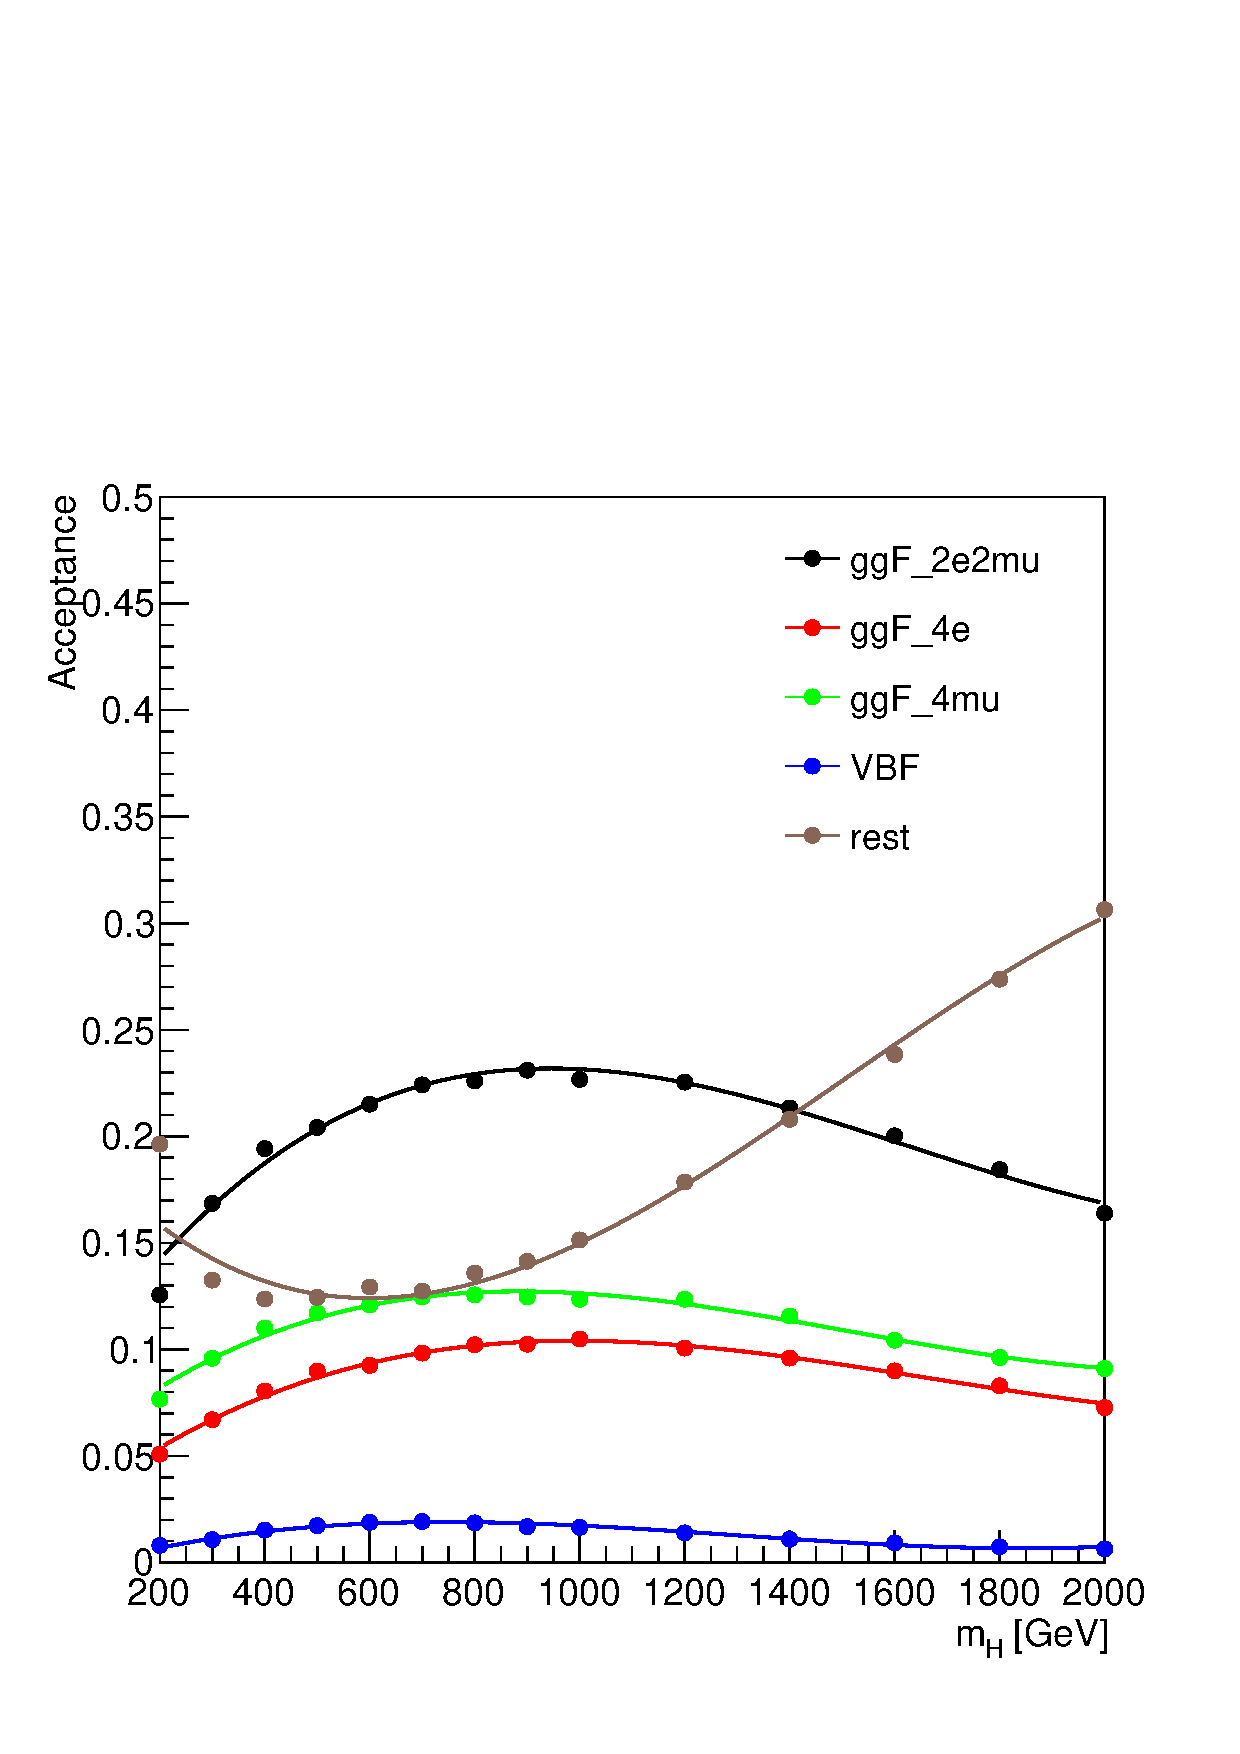
\includegraphics[width=0.43\textwidth]{figures/HMHZZ/selection/acc_dnn_ggF.pdf}}
\subfloat[]{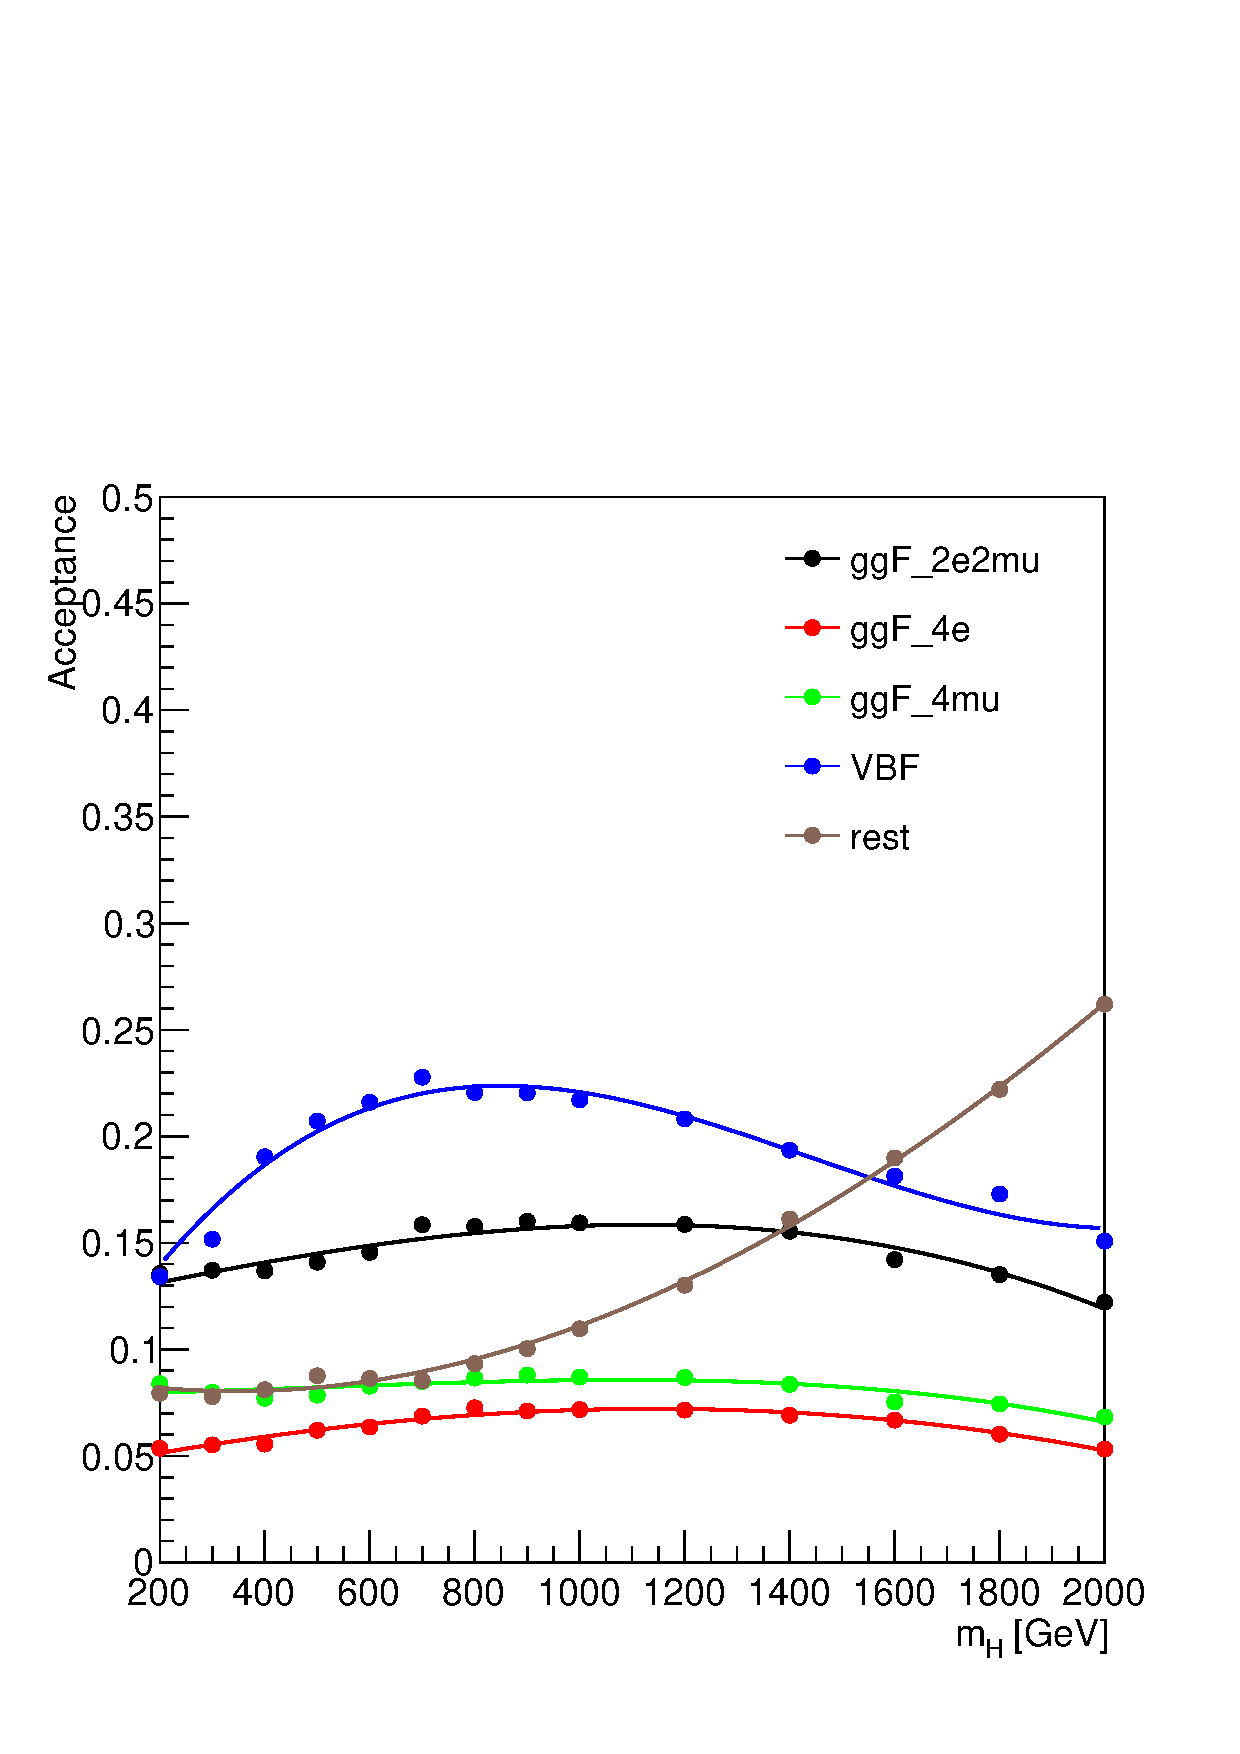
\includegraphics[width=0.43\textwidth]{figures/HMHZZ/selection/acc_dnn_VBF.pdf}}\\
\caption{NWA acceptance as a function of $m_{H}$ for the MVA-based categorization for the samples of
(a) ggF production;
(b) VBF production. 
}
\label{fig:hmhzz_acc_dnn}
\end{figure}

\begin{figure}[h]
\centering
\subfloat[]{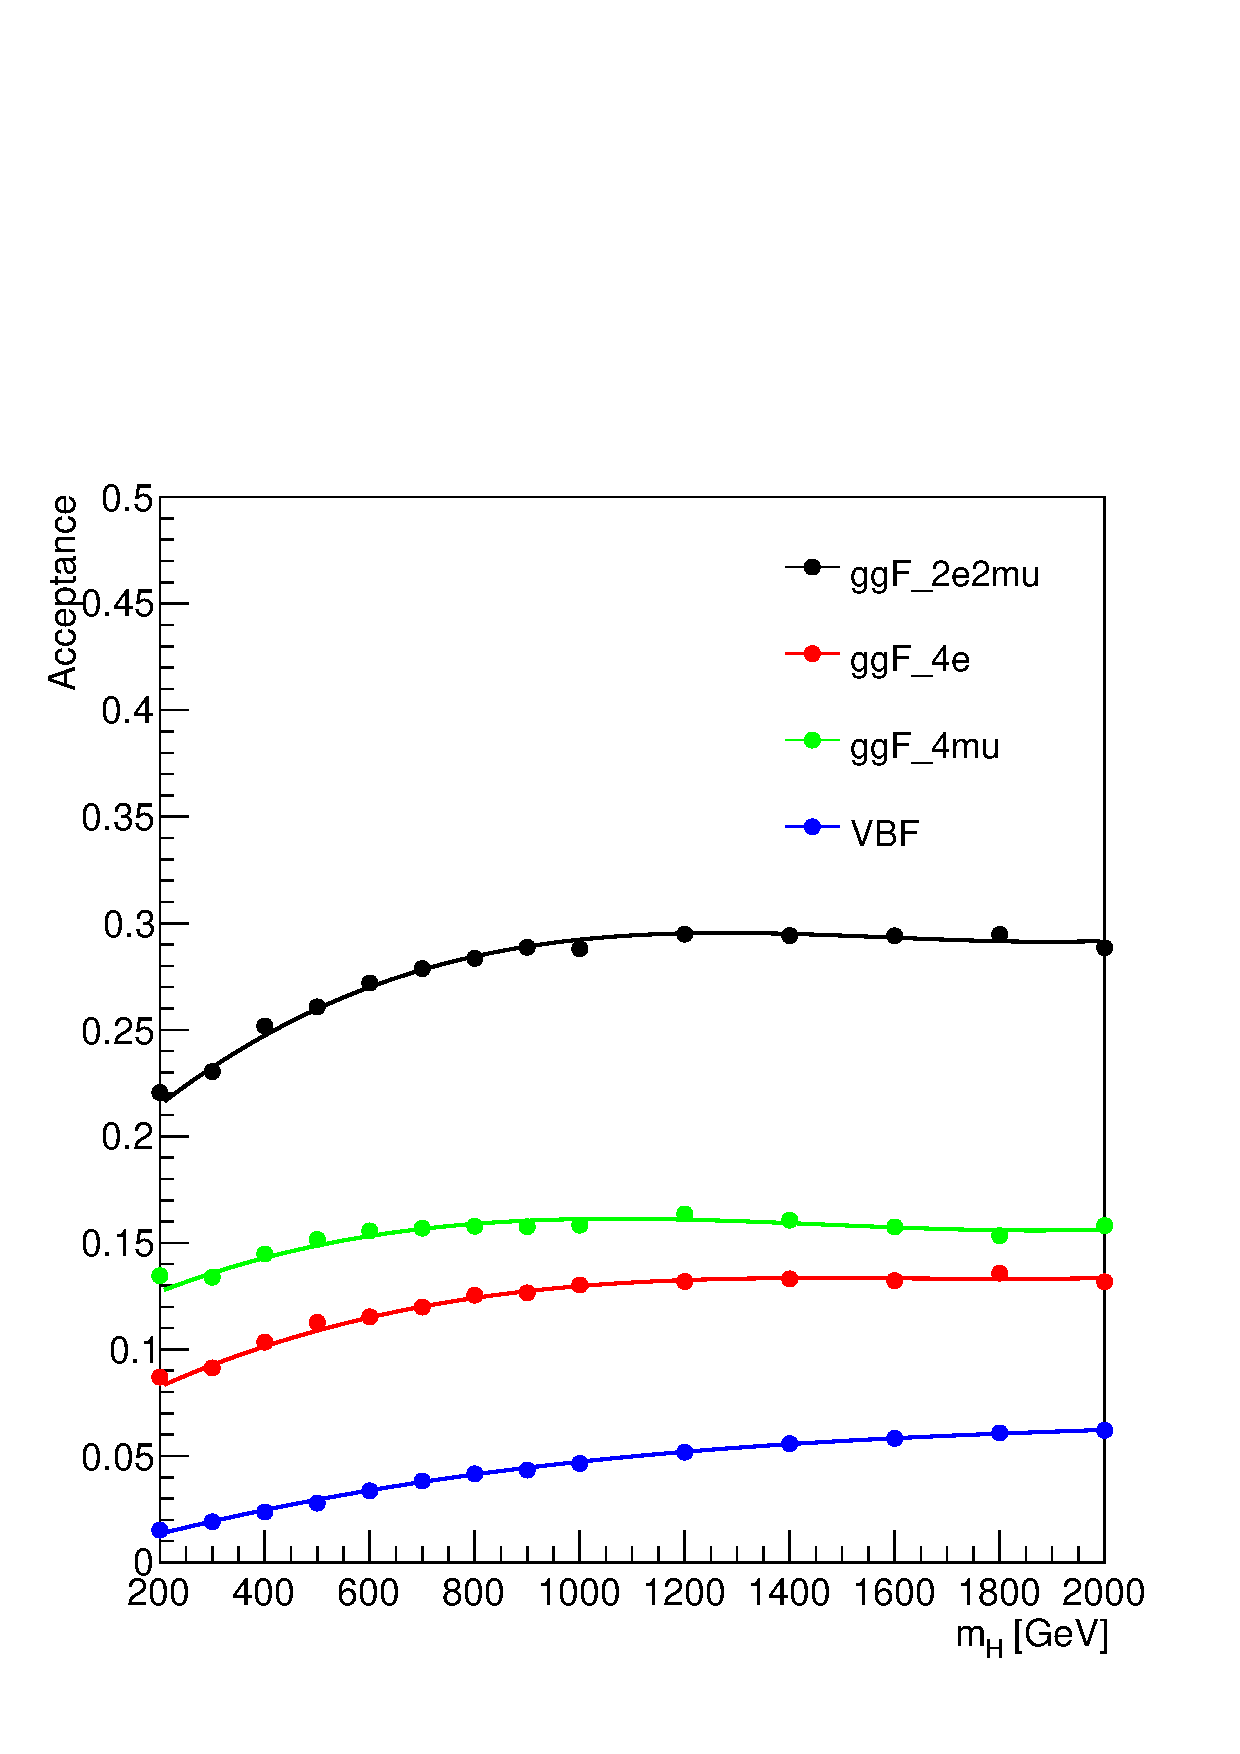
\includegraphics[width=0.43\textwidth]{figures/HMHZZ/selection/acc_cut_ggF.pdf}}
\subfloat[]{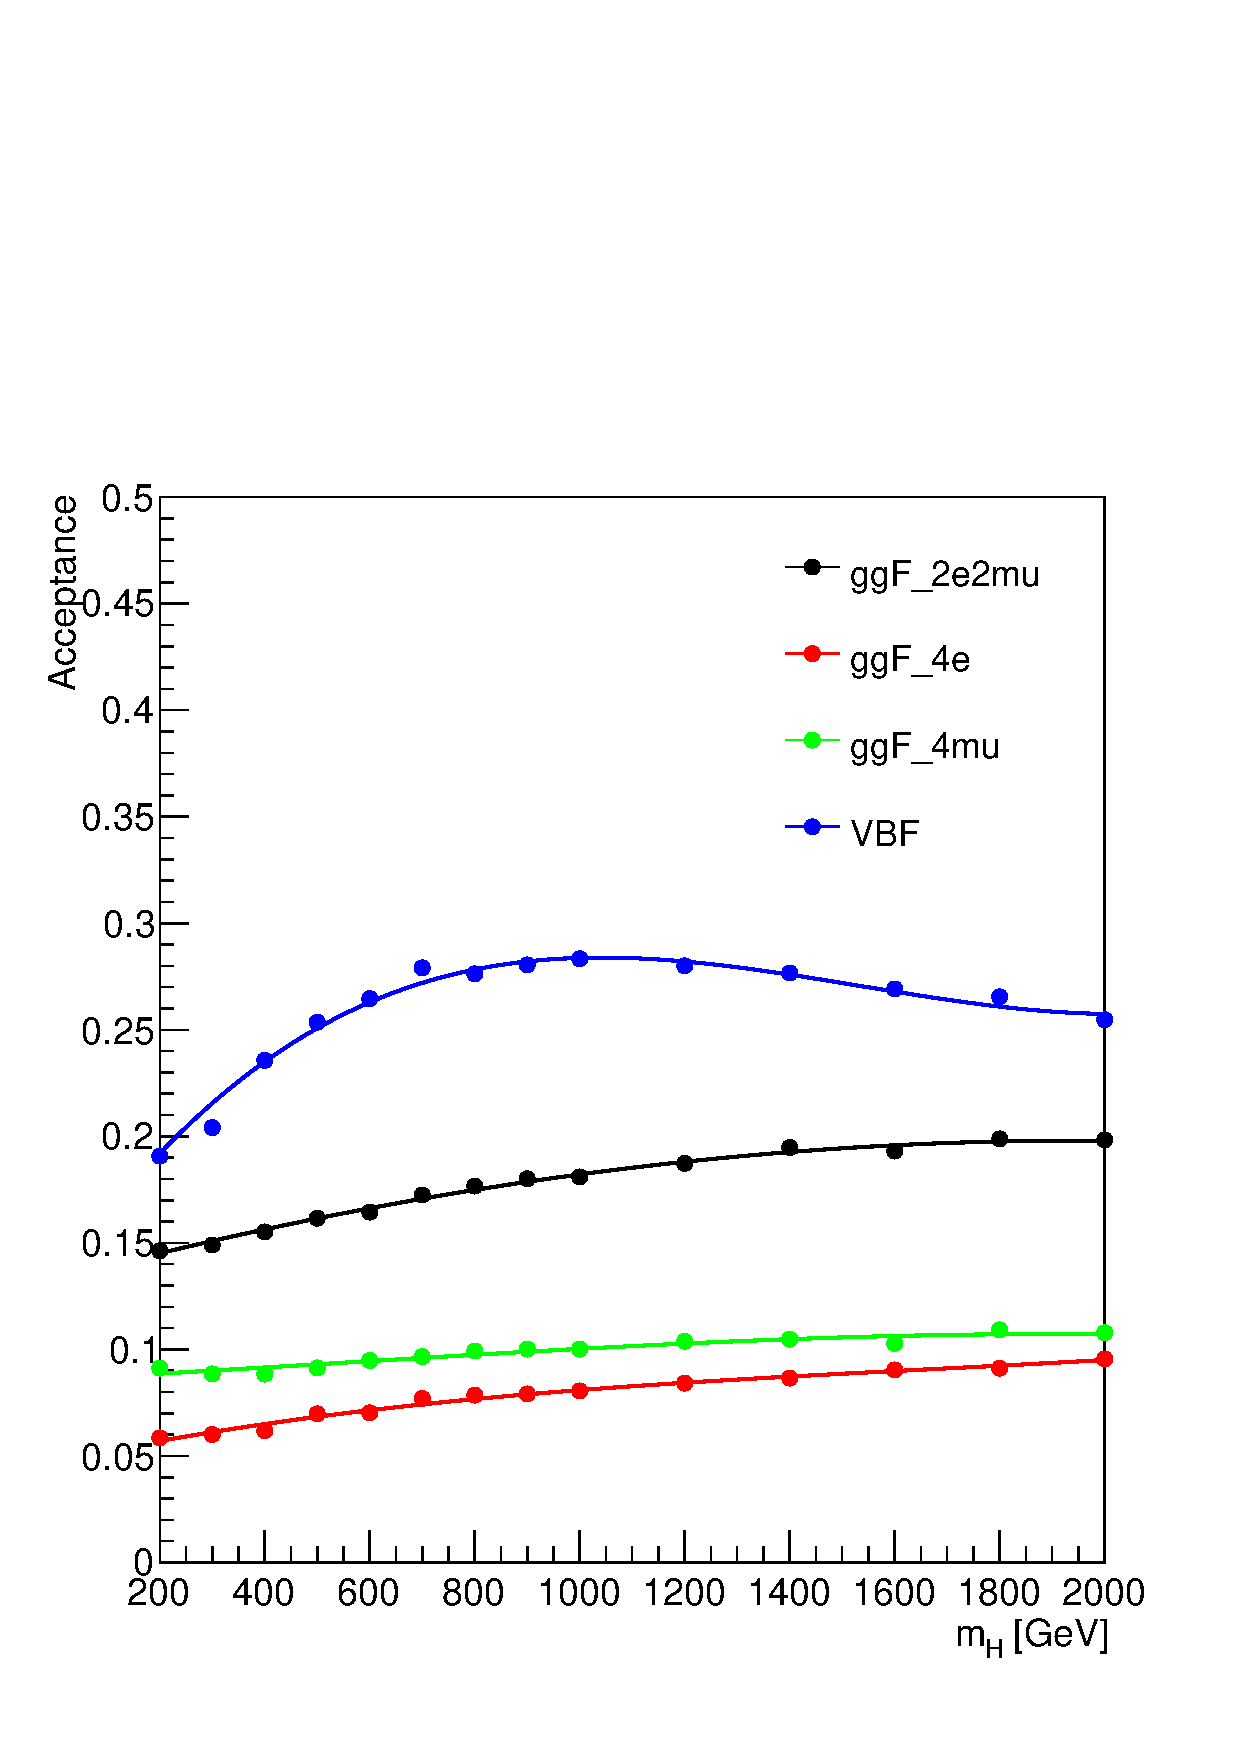
\includegraphics[width=0.43\textwidth]{figures/HMHZZ/selection/acc_cut_VBF.pdf}}\\
\caption{NWA acceptance as a function of $m_{H}$ for the Cut-based categorization for the samples of
(a) ggF production mode;
(b) VBF production mode. }
\label{fig:hmhzz_acc_cut}
\end{figure}
